\chapter{面向ASIC的自动化近似乘法器设计方法}

\section{引言}

许多近似乘法器在设计时都有一个隐含的假设,即乘数和被乘数都是均匀分布的,然而很多应用并不满足该假设。例如,文献\cite{DNN:WeightAnalysis2}发现深度神经网络(Deep Neural Network, DNN)中权重的分布并不是均匀的,而是集中在某个值附近。同时,近似乘法器通常是不对称的,这意味着交换输入前后乘法器的输出结果不一致。现有的近似乘法器设计方法没有同时考虑数据分布和输入极性,无法充分利用不同应用的数据统计学特性,生成高性能的近似乘法器。因此本章首先分析了这两个因素对乘法器精度的影响,之后提出了一个基于数据分布和输入极性的自动化近似乘法器设计方法,能够高效地生成适用于给定应用的高质量近似乘法器,提高计算效率。


\section{数据分布和输入极性对近似乘法器精度的影响}

假设一个近似乘法器在输入为$x$、$y$时输出为$f(x,y)$,由式\eqref{AC:Arith:ED}得该输入下误差距离ED的平方为:
\begin{equation}
    ED^2 = ( \ xy - f(x,y) \ ) ^2
\label{AC:AM:Adapt:Eq:ED2}
\end{equation}
若将该近似乘法器应用于某一特定应用,且经统计该应用中乘法的两个输入分布为$p_1$和$p_2$,由式\eqref{AC:Arith:MSE}和式\eqref{AC:AM:Adapt:Eq:ED2}得均方误差MSE为:
\begin{align}
    & MSE = \sum_{i=0}^{N-1} \sum_{j=0}^{M-1} ( \ x_i y_j - f(x_i,y_j) \ ) ^2 p(x^{\prime}_i, y^{\prime}_j) \label{AC:AM:Adapt:Eq:MSE} \\
    & p(x^{\prime}_i, y^{\prime}_j) = \left\{
        \begin{aligned}
          p_1(x_i) \cdot p_2(y_j),\ \ x^{\prime}_i=x_i\ \text{且}\ y^{\prime}_j=y_j. \\
          p_1(y_j) \cdot p_2(x_i),\ \ x^{\prime}_i=y_j\ \text{且}\ y^{\prime}_j=x_i.
        \end{aligned}
        \right.      \label{AC:AM:Adapt:Eq:pxy}
\end{align}
式中 $x_i \in \{x_0, x_1, \cdots , x_{N-1}\}$, $y_j \in \{y_0, y_1, \cdots , y_{M-1}\}$,常数$N$和$M$分别是$x$和$y$的所有可能输入情况的总数,式\eqref{AC:AM:Adapt:Eq:pxy}代表交换乘法器输入带来的影响。

\subsection{数据分布的影响}

\begin{figure}[!htb]
    \centering
    \subfigure[输入分布直方图]{
    \label{DNN:LeNet_MNIST:Fig:FC1_data}
    \begin{minipage}[t]{0.48\linewidth}
    \centering
    \includegraphics[width=\linewidth]{./figs/DNN-LeNet_MNIST_FC1_input.pdf}
    \end{minipage}
    }
    \subfigure[权重分布直方图]{
    \label{DNN:LeNet_MNIST:Fig:FC1_weight}
    \begin{minipage}[t]{0.48\linewidth}
    \centering
    \includegraphics[width=\linewidth]{./figs/DNN-LeNet_MNIST_FC1_weight.pdf}
    \end{minipage}
    }
    \centering
    \caption{采用8比特位宽量化的LeNet网络在MNIST数据集上训练后FC1层的输入和权重的数据分布直方图}
\label{DNN:LeNet_MNIST:Fig:FC1_distribution}
\end{figure}

为了证明不同数据分布对近似乘法器精度的影响,将文献\cite{AC:AM:OU}提出的面向浮点数乘法器的设计方法拓展到定点数领域,针对均匀分布和从DNN应用中提取的真实分布分别生成了8比特无符号整数近似乘法器$f^{(1)}$和$f^{(2)}$并进行误差比较,过程如下:

对于均匀分布,易得$f^{(1)} = -16384 + 128 x + 128 y$,是一个对称的乘法器。对于DNN应用,为了获得操作数的概率分布,对采用8比特位宽无符号整数量化(Quantization)的LeNet网络在MNIST数据集上进行训练\cite{DNN:LeNet_MNIST},统计第一个全连接(First Fully-Connected, FC1)层的特征输入和权重的数据分布,如图\ref{DNN:LeNet_MNIST:Fig:FC1_distribution}所示,可以看到输入值很多是0而权重值集中在128附近。
将输入和权重分别用半高斯和高斯分布进行拟合,利用文献\cite{AC:AM:OU}的方法,可以得到$f^{(2)} = -1549 + 129 x + 12 y$。注意$f^{(2)}$是非对称的,$x$是特征输入,$y$是权重。

\begin{figure}[!htb]
    \centering
    \subfigure[$f^{(1)}$的误差分布图]{
    \label{AC:AM:Adapt:Fig:f1_ED2_dist}
    \begin{minipage}[t]{0.48\linewidth}
    \centering
    \includegraphics[width=\linewidth]{./figs/AC-AM-Adapt-f1_ED2_dist.png}
    \end{minipage}
    }
    \subfigure[$f^{(2)}$的误差分布图]{
    \label{DNN:Fig:f2_ED2_dist}
    \begin{minipage}[t]{0.48\linewidth}
    \centering
    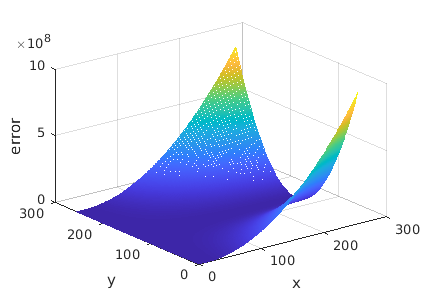
\includegraphics[width=\linewidth]{./figs/AC-AM-Adapt-f2_ED2_dist.png}
    \end{minipage}
    }
    \centering
    \caption{近似乘法器$f^{(1)}$和$f^{(2)}$的误差分布图,这里的误差是指误差距离ED的平方}
\label{AC:AM:Adapt:Fig:f1_f2_ED2_dists}
\end{figure}

近似乘法器$f^{(1)}$和$f^{(2)}$的误差分布如图\ref{AC:AM:Adapt:Fig:f1_f2_ED2_dists}所示,这里的误差是由式\eqref{AC:AM:Adapt:Eq:ED2}计算得到的,可以看到$f^{(2)}$在$x=0$、$y=128$附近的误差比$f^{(1)}$小。把FC1中的精确乘法分别全部替换为$f^{(1)}$和$f^{(2)}$,重新对LeNet进行训练,并把每一次乘法产生的误差(误差距离ED的平方)相加,得到$f^{(1)}$的总误差为$3.12 \times 10^{16}$,$f^{(2)}$的总误差为$4.77 \times 10^{14}$,比$f^{(1)}$小两个数量级,这充分说明了在设计近似乘法器时考虑真实数据分布的重要性。

\subsection{输入极性的影响}

为了展示输入极性对近似乘法器精度的影响,对基于CGP方法开发的包含500个帕累拖最优(Pareto optimality)的近似乘法器库Evoapprox8b\cite{AC:AM:CGP_Evoapprox8b}进行了研究,过程如下:

假设近似乘法器的输入分别是$x$和$y$,对于DNN或滤波器(Filter)应用,定义$P=0$代表$x$是输入、$y$是权重,$P=1$代表$x$是权重、$y$是输入。基于LeNet网络和MNIST数据集\cite{DNN:LeNet_MNIST},对Evoapprox8b\cite{AC:AM:CGP_Evoapprox8b}中全部的500个近似乘法器进行$P=0$和$P=1$的精度评估,结果如图\ref{AC:AM:Adapt:Fig:Evo8_accuracy_P}所示。
\begin{figure}[!htb]
    \centering
    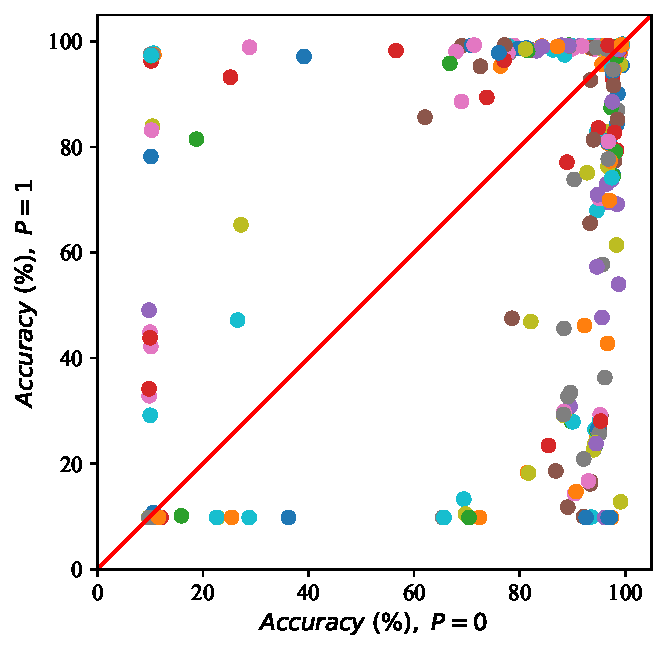
\includegraphics[width=0.7\linewidth]{./figs/AC-AM-Adapt-Evo8_accuracy_P.pdf}
    \caption{基于LeNet和MNIST得到的Evoapprox8b中全部500个乘法器在$P=0$和$P=1$的情况下的精度散点图}
    \label{AC:AM:Adapt:Fig:Evo8_accuracy_P}
\end{figure}
在图\ref{AC:AM:Adapt:Fig:Evo8_accuracy_P}中,每个点代表一个近似乘法器,横轴表示$P=0$时的精度,纵轴表示$P=1$时的精度,落在红线上的点代表该乘法器在交换输入后LeNet的精度保持不变。可以看到,落在红线上的点很少,这意味着交换输入会对大多数近似乘法器的精度产生影响。同时,点离红线的距离代表了乘法器不对称的程度,距离越远,乘法器在该DNN下的不对称程度越高,交换输入后对精度的影响越大。易知图\ref{AC:AM:Adapt:Fig:Evo8_accuracy_P}中点离红线的距离$D$为:
\begin{equation}
    \label{AC:AM:Adapt:Eq:Evo8_D}
      D =  100 \times | A_{P_0} - A_{P_1} |
\end{equation} 
式中$A_{P_0}$和$A_{P_1}$分别表示该点在$P=0$和$P=1$时的精度,$| A_{P_0} - A_{P_1} |$代表两个精度的差值的绝对值。图\ref{AC:AM:Adapt:Fig:Evo8_D}展示了图\ref{AC:AM:Adapt:Fig:Evo8_accuracy_P}中全部的500个点与红线的距离直方图,
\begin{figure}[!ht]
    \centering
    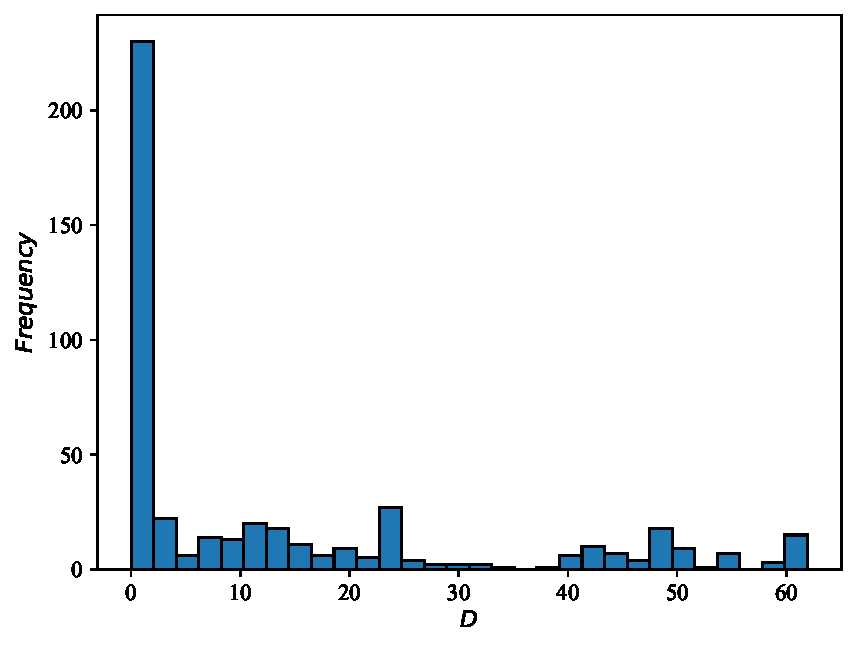
\includegraphics[width=0.7\linewidth]{./figs/AC-AM-Adapt-Evo8_D.pdf}
    \caption{Evoapprox8b中全部500个乘法器不对称程度统计直方图}
    \label{AC:AM:Adapt:Fig:Evo8_D}
\end{figure}
结果表明超过250个点的$D$大于2.8,这意味着Evoapprox8b\cite{AC:AM:CGP_Evoapprox8b}中超过一半的乘法器的精度在交换输入前后至少相差2.8\%。值得注意的是所有乘法器的精度评估均基于网络规模较小的LeNet,当网络规模上升后,考虑到误差的累计,由近似乘法器的不对称性引起的精度下降会更加严重,这充分说明了在设计近似乘法器时考虑输入极性的重要性。

% \section{研究内容与创新点}

% 本文提出了一种新的自动化近似乘法器生成方法,受文献\cite{AC:AM:SDLC}的启发,该方法通过逻辑操作和移位操作在部分积生成后、累加前对部分积进行了一次压缩,降低部分积阵列的规模,减轻后续的累加压力。同时,与文献\cite{AC:AM:SDLC}只采用或操作不同,本文提出的方法同时利用与、或、异或和移位操作对部分积进行压缩,降低乘法器的误差。最后,该方法将设计近似乘法器的问题建模成数学问题,利用计算机自动寻找在给定输入分布下的最优压缩操作,同时考虑输入极性,主要创新点如下:
% \begin{itemize}
%     \item 为了方便测试不同近似乘法器在不同规模神经网络上的性能,本文提出并开源了一个基于8比特无符号数量化的DNN推断(Inference)精度评估工具,该工具将一个近似乘法器表示为一个查找表并对网络中的精确乘法进行替换,支持LeNet\cite{DNN:LeNet_MNIST}、AlexNet\cite{DNN:AlexNet}、VGG16\cite{DNN:VGG16}三个不同规模的神经网络和MNIST\cite{DNN:LeNet_MNIST}、CIFAR-10\cite{DNN:CIFAR-10}两个数据集。
%     \item 提出的设计方法可以生成任意分布下的无符号乘法器,针对8比特位宽的三个不同规模的神经网络的实验结果表明,与国际前沿工作相比,生成的近似乘法器在几乎没有精度损失的情况下,功耗延迟面积积(Product of Power, Delay, and Area,缩写作PDA)提升了26.4\%。同时,针对大规模神经网络设计的近似乘法器在面对小规模神经网络时表现出了一定的可迁移性。
%     \item 利用改进的Baugh-Wooley算法\cite{EM:baugh-wooley,EM:baugh-wooley_modified_PP_reorga,EM:baugh-wooley_diff}(见\ref{改进的Baugh-Wooley算法}),方法能够生成补码有符号乘法器,基于16比特位宽的有限冲击响应(Finite Impulse Response, FIR)滤波器的实验结果表明,与国际前沿工作相比,生成的近似乘法器在几乎没有任何精度损失的情况下,PDA优化了27.1\%。
% \end{itemize}

\section{同时考虑分布和极性的设计方法}

受相关工作\cite{AC:AM:SDLC,AC:AM:OU,AC:AM:CGP_2016}的启发,对乘法器的部分积在生成后、累加前同时利用多种操作对其进行压缩,降低部分积阵列的规模,减轻后续的累加压力。与文献\cite{AC:AM:SDLC}只采用或操作不同,本文提出的方法同时利用与、或、异或和移位操作对部分积进行压缩,降低乘法器的误差。最后,把寻找最优压缩操作的问题建模成数学问题,利用计算机自动寻找在给定输入分布下的最优压缩操作,同时考虑输入极性。

\subsection{无符号乘法器}
\begin{figure}[ht]
    \centering
    \subfigure[4$\times$4无符号乘法器的部分积阵列(压缩前)]{
    \label{AC:AM:Adapt:Fig:4x4_unsigned_PP_array_orig}
    \begin{minipage}[t]{0.45\linewidth}
    \centering
    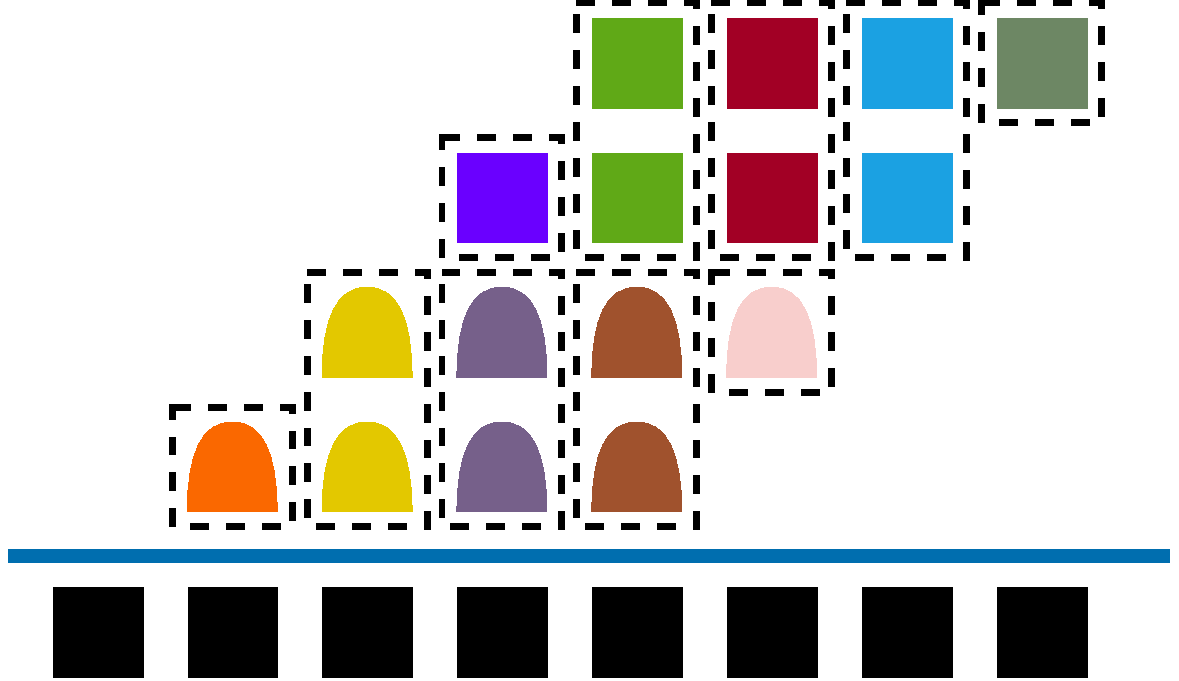
\includegraphics[width=\linewidth]{./figs/AC-AM-Adapt-4x4_unsigned_PP_array_orig.pdf}
    \end{minipage}
    }
    \subfigure[4$\times$4无符号乘法器的部分积阵列(压缩后)]{
    \label{AC:AM:Adapt:Fig:4x4_unsigned_PP_array_compressed}
    \begin{minipage}[t]{0.45\linewidth}
    \centering
    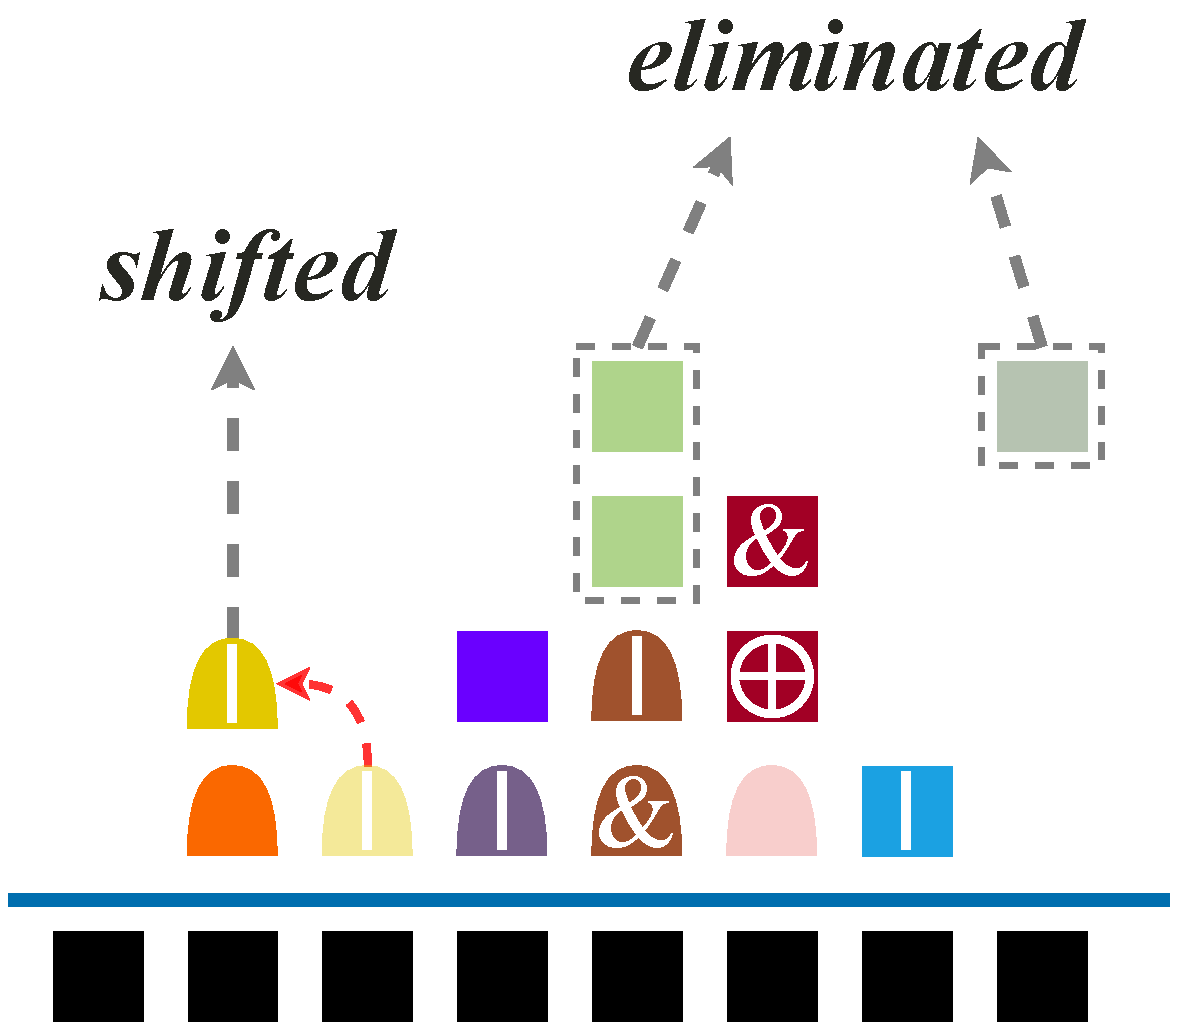
\includegraphics[width=\linewidth]{./figs/AC-AM-Adapt-4x4_unsigned_PP_array_compressed.pdf}
    \end{minipage}
    }
    \caption{利用AND、OR、XOR、shift操作对4$\times$4无符号乘法器部分积进行压缩的示例}
    \label{AC:AM:Adapt:Fig:4x4_unsigned}
\end{figure}

图\ref{AC:AM:Adapt:Fig:4x4_unsigned}展示了一个利用与、或、异或和移位共4种操作对4$\times$4无符号乘法器部分积进行压缩的示例,在图\ref{AC:AM:Adapt:Fig:4x4_unsigned_PP_array_orig}中,蓝线上方不同颜色的正方形或半椭圆形代表部分积比特,组成部分积阵列,共由$4^2$个与门生成。首先,选择全部四行部分积,每两行一组对其权重相同的部分积比特进行分簇,共分为10个簇,每个簇由虚线矩形表示,包含1个或2个比特;之后,利用与、或、异或和移位操作对簇内的部分积进行运算,生成运算后的新比特(可能有多个),运算共有6个:单独地与、或、异或三种逻辑操作,以及分别三种逻辑操作后左移一位。运算过程中有以下几点需要注意:(1)簇可以直接消失;(2)对只包含一个部分积比特的簇(以下简称为单比特簇),不进行运算,只存在保留或消失两种情况;(3)对包含两个比特的簇(以下简称为双比特簇),若没消失,则该簇不同运算产生的部分积比特可能会同时存在。

把双比特簇运算产生的比特(可能有多个)和单比特簇保留产生的比特统称为压缩项(Compressed term),
图\ref{AC:AM:Adapt:Fig:4x4_unsigned_PP_array_compressed}展示了对图\ref{AC:AM:Adapt:Fig:4x4_unsigned_PP_array_orig}中的部分积阵列进行压缩的一种可能结果,蓝线以上的所有形状代表压缩项,组成了新的部分积阵列。
对于内有符号的压缩项,其符号代表了对图\ref{AC:AM:Adapt:Fig:4x4_unsigned_PP_array_orig}中与压缩项同颜色的双比特簇执行的逻辑操作,注意逻辑操作后可能会伴随移位。另外,从图\ref{AC:AM:Adapt:Fig:4x4_unsigned_PP_array_compressed}中可以看到有两个簇消失了。

假设精确乘法器的部分积阵列有$g$行,每行有$h$个比特,选择$l$行部分积进行分簇,则未分簇的部分积比特的个数$S$为:
\begin{align}
        & S = ( g - l ) h, \ \ \ l \in \{0, 2, 4, \cdots, g^{\prime} \} \label{AC:AM:Adapt:Eq:unsigned_S}, \\
        & g^{\prime} = \left\{
    \begin{aligned}
      g, \ \ \  & \ \ \ \ \ g \text{是偶数}. \\
      g - 1, & \ \ \ \ \ g \text{是奇数}.
    \end{aligned}
  \right.
  \label{AC:AM:Adapt:Eq:unsigned_g}
\end{align}
例如,对图\ref{AC:AM:Adapt:Fig:4x4_unsigned_PP_array_orig}有$g=h=l=4$,$S=0$。

\subsection{有符号乘法器}

\begin{figure}[ht]
    \centering
    \subfigure[改进的4$\times$4 Baugh-Wooley乘法器的部分积阵列(压缩前)]{
    \label{AC:AM:Adapt:Fig:4x4_signed_PP_array_orig}
    \begin{minipage}[t]{0.45\linewidth}
    \centering
    \includegraphics[width=\linewidth]{./figs/AC-AM-Adapt-4x4_signed_PP_array_orig.pdf}
    \end{minipage}
    } \ \ \ 
    \subfigure[改进的4$\times$4 Baugh-Wooley乘法器的部分积阵列(压缩后)]{
    \label{AC:AM:Adapt:Fig:4x4_signed_PP_array_compressed}
    \begin{minipage}[t]{0.45\linewidth}
    \centering
    \includegraphics[width=\linewidth]{./figs/AC-AM-Adapt-4x4_signed_PP_array_compressed.pdf}
    \end{minipage}
    }
    \caption{利用AND、OR、XOR、shift操作对改进的4$\times$4 Baugh-Wooley乘法器的部分积进行压缩的例子}
    \label{AC:AM:Adapt:Fig:4x4_signed}
\end{figure}

两个部分积比特成双比特簇的前提是两者具有相同的权重值,补码有符号数直接相乘产生的部分积比特的权重值有正有负,无法直接进行分簇,改进的Baugh-Wooley算法\cite{EM:baugh-wooley,EM:baugh-wooley_modified_PP_reorga,EM:baugh-wooley_diff}(见\ref{改进的Baugh-Wooley算法})能够将所有部分积比特的权重变为正值,顺利实现分簇压缩。有符号乘法器部分积的压缩过程与无符号乘法器类似,图\ref{AC:AM:Adapt:Fig:4x4_signed}展示了一个利用提出的4种操作对改进的Baugh-Wooley乘法器的部分积进行压缩的示例,与图\ref{AC:AM:Adapt:Fig:4x4_unsigned}相比有以下不同:
\begin{itemize}
    \item 改进的Baugh-Wooley乘法器的部分积比特并不全部由与门生成,有些由与非(NAND)门产生,在图\ref{AC:AM:Adapt:Fig:4x4_signed_PP_array_orig}中,蓝线上方每个正方形代表一个部分积比特,内有“N”符号的正方形表示该比特由与非门生成,第一行部分积和最后一行部分积中标有“1”符号的正方形代表添加的两个常数“1”。
    \item 与图\ref{AC:AM:Adapt:Fig:4x4_unsigned_PP_array_orig}选择全部4行部分积进行分簇压缩不同,图\ref{AC:AM:Adapt:Fig:4x4_signed_PP_array_orig}只选择了前两行部分积进行压缩,后两行部分积保持不变。与选择全部的部分积进行压缩相比,这能够提高生成的近似乘法器的精度,即可以通过调整分簇的部分积的行数来生成具有不同质量的近似乘法器,注意最后一行部分积的常数“1”永远不参与压缩。
    \item 图\ref{AC:AM:Adapt:Fig:4x4_unsigned_PP_array_compressed}中全部的压缩项组成了新的部分积阵列,而图\ref{AC:AM:Adapt:Fig:4x4_signed_PP_array_compressed}中压缩项和原先未分簇的部分积一起构成了新的部分积阵列。
\end{itemize}

在不考虑额外添加的两个常数“1”的情况下,同样假设改进的Baugh-Wooley乘法器有$g$行部分积,每行有$h$个部分积比特,选择$l$行部分积进行分簇压缩,式\eqref{AC:AM:Adapt:Eq:unsigned_S}变为:
\begin{equation}
    \label{AC:AM:Adapt:Eq:signed_S}
        S = \left\{
          \begin{aligned}
            gh + 2, \ \ \ & \ \ \ l = 0, \\
            (g - l)h + 1, & \ \ \ l \in \{2, 4, \cdots, g^{\prime} \},
          \end{aligned}
          \right.
\end{equation}
式中$g^{\prime}$如式\eqref{AC:AM:Adapt:Eq:unsigned_g}所示。对于图\ref{AC:AM:Adapt:Fig:4x4_signed_PP_array_orig},$ h = g = g^{\prime} = 4 $,$ l = 2 $,因此$ S = 9 $。


\subsection{自动化求解}

当输入为$x_i$、$y_j$时,本文提出的基于部分积压缩的近似乘法器的输出可以被公式化地表述为:
\begin{equation}
\label{AC:AM:Adapt:Eq:f}
    f(x_i, y_j \vert \boldsymbol{\theta}) =  \sum\limits_{u=0}^{S-1} b_u + \sum\limits_{k=0}^{Z-1} \theta_k L_k
\end{equation}
式中$b_u$表示$S$个不分簇的部分积比特中的一个;$\theta_k \in \{0, 1\}$,代表是否存在一个压缩项;$L_K$代表对一个双比特簇执行一种运算或对一个单比特簇进行保留;$Z$是待求解的变量的数目,也代表压缩项总数的上限。例如,在无符号乘法器中,每两行部分积包含2个单比特簇和$h-1$个双比特簇,因此,当选择$l$行部分积进行压缩时,无符号乘法器的$Z$为:
\begin{equation}
    \label{AC:AM:Adapt:Eq:Z_unsigned}
      Z = [2 \times 1 + (h-1) \times 6] \times \frac{l}{2} = (3h-2)l
      %  \ \ \ l \in \{0, 2, 4, \cdots, g^{\prime} \}.
\end{equation}

对基于改进的Baugh-Wooley算法的有符号乘法器,其部分积阵列中的第一行中有一个额外的常数“1”(如图\ref{AC:AM:Adapt:Fig:4x4_signed_PP_array_orig}所示),因此前两行部分积包含1个单比特簇和$h$个双比特簇,$Z$变为:
\begin{equation}
    \label{AC:AM:Adapt:Eq:Z_signed}
        Z = \left\{
          \begin{aligned}
            0 , \ \ \ \ \ \  & \ \ \ \ l = 0, \\
            (3h-2)l + 5, & \ \ \ \  l \in \{2, 4, \cdots, g^{\prime} \}.
            \end{aligned}
          \right.
\end{equation}
式中$g^{\prime}$如式\eqref{AC:AM:Adapt:Eq:unsigned_g}所示,注意最后一行部分积的常数“1”永远不参与分簇。

\begin{figure}[!ht]
    \centering
    \includegraphics[width=0.3\linewidth]{./figs/AC-AM-Adapt-2x2_unsigned_PP_array_orig.pdf}
    \caption{$2\times2$无符号乘法器的部分积阵列及$S = 0$时的分簇情况}
    \label{AC:AM:Adapt:Fig:2x2_unsigned_PP_array_ori}
\end{figure}

图\ref{AC:AM:Adapt:Fig:2x2_unsigned_PP_array_ori}展示了$2\times2$无符号乘法器的部分积阵列及$S = 0$时的分簇情况,式\eqref{AC:AM:Adapt:Eq:f}变为:
\begin{align}
      f(x_i, y_j \vert \boldsymbol{\theta}) = 0 
       &\ + \theta_0 P_0 \cdot 2^0 \notag \notag \\
       &\ + \theta_1 ( P_1 \& P_2 ) \cdot 2^1 + \theta_2 ( P_1 \& P_2 ) \cdot 2^2 \notag \\
       &\ + \theta_3 ( P_1 | P_2 ) \cdot 2^1 + \theta_4 ( P_1 | P_2 ) \cdot 2^2 \notag \\
       &\ + \theta_5 ( P_1 \oplus P_2 ) \cdot 2^1 + \theta_6 ( P_1 \oplus P_2 ) \cdot 2^2 \notag \\
       &\ +\theta_7 P_3 \cdot 2^2
       \label{AC:AM:Adapt:Eq:2x2_unsigned_f}
\end{align}

对于式\eqref{AC:AM:Adapt:Eq:f},任意的$Z$,均存在$\boldsymbol{\theta} = \boldsymbol{{\theta}^{e}}$使$f(x_i, y_j \vert \boldsymbol{{\theta}^{e}}) =  x_i \times y_j$对任意的$x_i \times y_j$成立,即对任意位宽的乘法器,不论选择几行部分积进行分簇压缩,精确乘法器都是所有可能压缩情况中的一个解。例如,$\boldsymbol{\theta} = [1, 0, 1, 0, 0, 1, 0, 1]$代表式\eqref{AC:AM:Adapt:Eq:2x2_unsigned_f}是一个精确的2$\times$2无符号乘法器,相当于对图\ref{AC:AM:Adapt:Fig:2x2_unsigned_PP_array_ori}在保留$P_0$和$P_3$的同时使用一个半加器对$P_1$和$P_2$进行累加。这表明所有可能的压缩情况构成了一个高质量的解空间,存在许多低误差的近似乘法器。

将式\eqref{AC:AM:Adapt:Eq:f}与式\eqref{AC:AM:Adapt:Eq:MSE}结合,以均方误差MSE为优化目标的求解问题可以被公式化地表示为:
\begin{equation}
    \label{AC:AM:Adapt:Eq:Obj_MSE}
      \mathop{min}\limits_{\boldsymbol{\theta}}\ \{ \sum_{i=0}^{N-1} \sum_{j=0}^{M-1} [(x_iy_j - (\sum\limits_{u=0}^{S-1} b_u + \sum\limits_{k=0}^{Z-1} \theta_k L_k) )^2  p(x^{\prime}_i, y^{\prime}_j) ] \}
      % \mathop{min}\limits_{}\boldsymbol{\theta}}\ [ \ E_d(X_d, Y_d, \boldsymbol{\theta}) + Cont(\boldsymbol{\theta}) \ ]
\end{equation}
式\eqref{AC:AM:Adapt:Eq:Obj_MSE}只考虑了误差,对近似乘法器来讲硬件开销也同样重要。
从电路实现角度来看,部分积阵列的规模与乘法器的性能强相关,为了降低压缩后新部分积阵列规模的大小,引入一个惩罚项$Cont(\boldsymbol{\theta})$作为优化目标的一部分,定义为:
\begin{align}
    Cont(\boldsymbol{\theta}) = \lambda T \label{AC:AM:Adapt:Eq:Cont} \\
    T = \sum_{k=0}^{Z-1} \theta_k \label{AC:AM:Adapt:Eq:T_exact}
\end{align}
其中$T$表示压缩项的总数,$\lambda$是一个用于控制惩罚程度的常量,$\lambda$越大,压缩项总数越少,新的部分积阵列规模越小,电路实现越简单,误差越大,反之则相反。
加入惩罚项后式\eqref{AC:AM:Adapt:Eq:Obj_MSE}变成了:
\begin{equation}
    \label{AC:AM:Adapt:Eq:Obj}
      \mathop{min}\limits_{\boldsymbol{\theta}}\ \{ \sum_{i=0}^{N-1} \sum_{j=0}^{M-1} [(x_iy_j - (\sum\limits_{u=0}^{S-1} b_u + \sum\limits_{k=0}^{Z-1} \theta_k L_k) )^2  p(x^{\prime}_i, y^{\prime}_j) ] +  Cont(\boldsymbol{\theta}) \}
      % \mathop{min}\limits_{}\boldsymbol{\theta}}\ [ \ E_d(X_d, Y_d, \boldsymbol{\theta}) + Cont(\boldsymbol{\theta}) \ ]
\end{equation}
即为最终的优化目标,式中$p(x^{\prime}_i, y^{\prime}_j)$代表乘法器的极性,由式\eqref{AC:AM:Adapt:Eq:pxy}给出。可采用混合整数遗传算法(Mixed
Integer Genetic Algorithm, MIGA)通过MATLAB或Python对式\eqref{AC:AM:Adapt:Eq:Obj}进行求解。

\subsection{求解过程}

求解过程包括以下三个步骤:(a)基于用户想要的面积减少比例$R$(与同位宽精确乘法器相比)来确定$l$的值,并根据式\eqref{AC:AM:Adapt:Eq:Obj_MSE}基于用户给定的输入分布生成具有不同输入极性的面向均方误差MSE的目标函数;(b)给定$R$,找到一个合适的$\lambda$值,根据式\eqref{AC:AM:Adapt:Eq:Obj}生成最终的两个输入极性相反的优化目标;(c)通过MIGA求解目标函数并生成近似乘法器。

\begin{figure}[!htb]
    \centering
    \subfigure[{$l=2, \;\; \lambda \in [500, \; 30000]$.}]{
    \label{}
    \begin{minipage}[t]{0.48\linewidth}
    \centering
    \includegraphics[width=\linewidth]{./figs/AC-AM-Adapt-8x8_unsigned_uniform_l2.pdf}
    \end{minipage}
    }
    \subfigure[{$l=4, \;\; \lambda \in [500, \; 30000]$.}]{
    \label{}
    \begin{minipage}[t]{0.48\linewidth}
    \centering
    \includegraphics[width=\linewidth]{./figs/AC-AM-Adapt-8x8_unsigned_uniform_l8.pdf}
    \end{minipage}
    }
    
    \subfigure[{$l=6, \;\; \lambda \in [200, \; 100000]$.}]{
    \label{}
    \begin{minipage}[t]{0.48\linewidth}
    \centering
    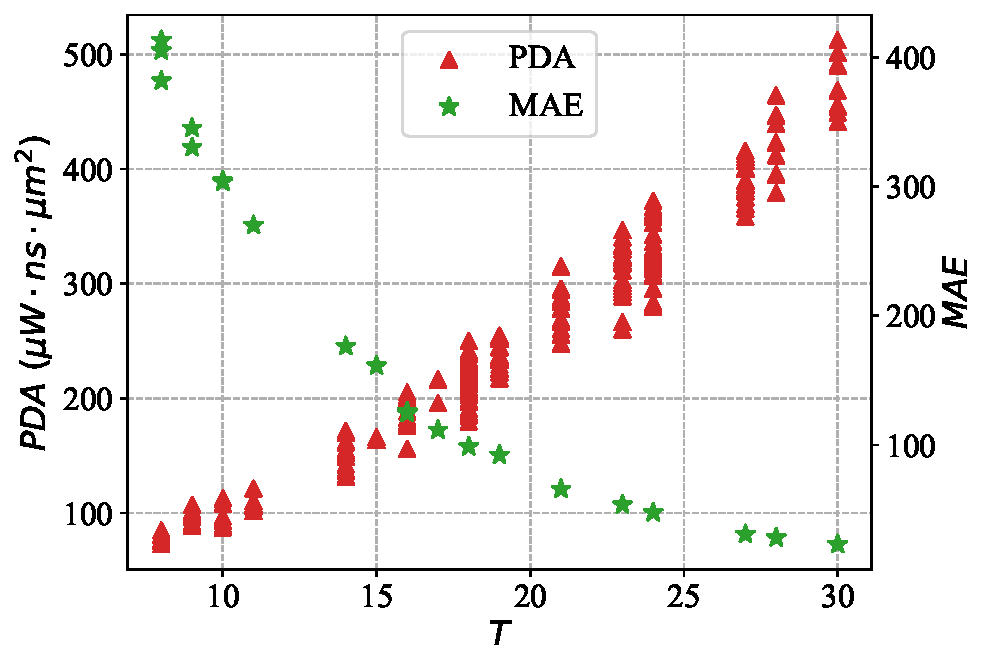
\includegraphics[width=\linewidth]{./figs/AC-AM-Adapt-8x8_unsigned_uniform_l6.pdf}
    \end{minipage}
    }
    \subfigure[{$l=8, \;\; \lambda \in [200, \; 100000]$.}]{
    \label{AC:AM:Adapt:8x8_unsigned_uniform_l8}
    \begin{minipage}[t]{0.48\linewidth}
    \centering
    \includegraphics[width=\linewidth]{./figs/AC-AM-Adapt-8x8_unsigned_uniform_l8.pdf}
    \end{minipage}
    }
    \centering
    \caption{均匀分布下8比特无符号乘法器在不同$l$和$\lambda$下得到的不同近似乘法器对应的压缩项总数$T$、乘法器的功耗延迟面积积PDA以及平均绝对误差MAE}
    \label{AC:AM:Adapt:8x8_unsigned_uniform_l2468}
\end{figure}

\subsubsection{根据用户想要的面积减少百分比$R$确定$l$}

在步骤(a)中,为了对任意的$R$确定一个合适的$l$值,对式\eqref{AC:AM:Adapt:Eq:Obj}测试了均匀分布下8比特无符号乘法器在不同$l$和$\lambda$下得到的不同近似乘法器对应的压缩项总数$T$(见式\eqref{AC:AM:Adapt:Eq:T_exact})、乘法器的功耗延迟面积积PDA以及平均绝对误差MAE(即平均误差距离MED,见式\eqref{AC:Arith:MED}),结果如图\ref{AC:AM:Adapt:8x8_unsigned_uniform_l2468}所示,
可以看到,当
\begin{equation}
    T \approx \frac{l-1}{2} h
\label{AC:AM:Adapt:Eq:T_approx}
\end{equation}
时,对应的乘法器能在精度和硬件之间取得一个较好的权衡,例如在图\ref{AC:AM:Adapt:8x8_unsigned_uniform_l8}中,$\dfrac{l-1}{2} h=28$,$T=29\text{或}30$。
% 假设,则生成的近似乘法器的面积正比于$S+\sum_{k=0}^{Z-1} \theta_k$。
假设乘法器的面积和部分积阵列的规模成正比,且任意位宽下生成的高质量近似乘法器的压缩项总数$T$都在$\dfrac{l-1}{2} h$附近,那么有:
\begin{equation}
    lh - ghR = \frac{l-1}{2} h
\end{equation}
则:
\begin{equation}
    l \approx \text{min} \{g^{\prime}, \; even ( 2gR-1 ) \}
\label{AC:AM:Adapt:Eq:l_approx}
\end{equation}
式中$even()$表示向上取最近的偶数。式\eqref{AC:AM:Adapt:Eq:l_approx}表示$l$为$\text{min} \{g^{\prime}, \; even ( 2gR-1 ) \}$时与合适的$\lambda$值一起能够在满足$R$的前提下产生高质量的解空间,实验结果表明式\eqref{AC:AM:Adapt:Eq:l_approx}能够指导生成高质量的近似乘法器。

式\eqref{AC:AM:Adapt:Eq:MSE}的计算需要遍历乘法器所有可能的输入情况,这对小位宽乘法器来讲是可行的,例如在Intel Xeon Platinum 8354H处理器上对8比特位宽乘法器利用单线程遍历($2^{16}$种输入情况)仅需15秒,对16比特位宽乘法器利用128线程遍历($2^{32}$种输入情况)需8小时,易知遍历时间随着乘法器位宽的增加指数增长,当位宽大于16比特时,遍历变得不可接受。有两种办法解决该问题:(1)如果实际应用中乘法器的输入只会取某些特定的值,并且遍历这些特定值的时间是可接受的,那么只需针对这些可能值进行计算;(2)当无法遍历所有可能输入值时,通过随机抽样的方式仅考虑一部分可能输入值进行计算。注意不论哪种情况都应基于真实的数据分布进行求解。

\subsubsection{根据用户想要的面积减少百分比$R$确定$\lambda$}

\begin{algorithm}[!]
    \caption{给定$R$找到一个合适的$\lambda$值}
    \label{AC:AM:Adapt:Alg:lambda}
    \KwIn { $R$:用户想要的面积减少比例$R$(与同位宽精确乘法器相比)。}
    \KwOut {$\lambda_R$:一个满足$R$并且能够生成高精度近似乘法器的$\lambda$的取值。}
    \BlankLine
    \textcolor{black}{
      MSE:均方误差,由式\eqref{AC:AM:Adapt:Eq:MSE}、式\eqref{AC:AM:Adapt:Eq:f}、式\eqref{AC:AM:Adapt:Eq:l_approx}和$R$联合确定; \\
      $Z$:由式\eqref{AC:AM:Adapt:Eq:Z_unsigned}或式\eqref{AC:AM:Adapt:Eq:Z_signed}联合式\eqref{AC:AM:Adapt:Eq:l_approx}、$R$确定; \\
      $\lambda_R = 1$; \  $T_{\lambda_R} = Z$; \ \ \ \ \ \ \ // 初始化 \\
      \While{$T_{\lambda_R} > \text{max}\{ lh - gh \times R, \; 0 \}$}{
        $\boldsymbol{\theta}^{\lambda_R}$ = MIGA($ MSE + \lambda_R \sum_{k=0}^{Z-1} \theta_k$); \ \ \ \ // 利用MIGA进行求解 \\
        $T_{\lambda_R} = \sum_{j=0}^{Z-1} \theta_j^{\lambda_R}$; \ \ \  \ \ \ \ \ // 压缩项总数 \\
        $\lambda_R = \lambda_R * 10$
      }
      \BlankLine
      $\lambda_R = \lambda_R \ / \ 20$; \\
      \Return{$\lambda_R$};}
  \end{algorithm}

给定$R$,$\lambda$的值可由算法\ref{AC:AM:Adapt:Alg:lambda}确定。在算法\ref{AC:AM:Adapt:Alg:lambda}中,对$\lambda$的取值从1开始尝试,若不满足条件直接将$\lambda$增大十倍,直到得到的解的压缩项总数$T$满足
\begin{equation}
    T \le lh -gh \times R 
\end{equation}
即认为$\lambda$的值和由式\eqref{AC:AM:Adapt:Eq:l_approx}确定的$l$一起满足$R$和式\eqref{AC:AM:Adapt:Eq:T_approx},能够生成高质量的近似乘法器。

需要注意的是,$R$是一种软性约束,即基于$R$按照式\eqref{AC:AM:Adapt:Eq:l_approx}和算法\ref{AC:AM:Adapt:Alg:lambda}得到的$l$和$\lambda$的值是指导性的,可在尝试后根据实际情况进行灵活调整。

\subsubsection{误差分析} \label{误差分析}

$l$与$\lambda$的取值和近似乘法器的精度高度相关,原因如下:
\begin{itemize}
    \item $\lambda$的大小影响生成的近似乘法器的压缩项总数,精确解($\boldsymbol{\theta} = \boldsymbol{{\theta}^{e}}$)对应的压缩项总数是一个适中的值,因此当$\lambda$较小时,目标函数由MSE主导,能够生成低误差的近似乘法器,反之$\lambda$较大时则会降低乘法器的精度;
    \item 对于给定的$g$和$h$,不分簇的部分积比特总数$S$与$l$成反比关系(见式\eqref{AC:AM:Adapt:Eq:unsigned_S}和式\eqref{AC:AM:Adapt:Eq:signed_S}),较小的$l$取值会导致大的$S$,能够在$\lambda$较大时也能产生低误差的近似乘法器,但坏处是硬件提升上限低;
    \item 对式\eqref{AC:AM:Adapt:Eq:Obj}的求解是一个NP难问题,尽管混合整数遗传算法MIGA提供了一个高效的求解思路,但MIGA的随机性则导致变量过多时求解效率不高。在式\eqref{AC:AM:Adapt:Eq:f}中,待求解的变量的数目$Z$的取值和$hl$成正比(见式\eqref{AC:AM:Adapt:Eq:Z_unsigned}和式\eqref{AC:AM:Adapt:Eq:Z_signed}),对于一个给定的$h$,大的$l$导致求解变量过多,MIGA算法无法高效对空间进行搜索。
\end{itemize}


\subsection{基于8比特无符号数量化的DNN推断精度评估工具}

本文提出并开源了一个面向近似乘法器的基于8比特无符号数量化的DNN推断精度评估工具,其中近似乘法器以查找表的形式表示。在该工具中,一个DNN通过有向无环图DAG进行表示,其中点代表DNN中的连接层,边代表数据流,当DAG中的一个节点被执行时,它的依赖项将被自动执行。图\ref{DNN:ApproxFlow:Fig:LeNet}展示了LeNet网络\cite{DNN:LeNet_MNIST}在工具中的DAG表示,一张图从Image节点输入,分类结果从FC2节点输出。

\begin{figure}[!ht]
    \centering
    \includegraphics[width=0.7\linewidth]{./figs/DNN-ApproxFlow_LeNet.pdf}
    \caption{LeNet在评估工具中的DAG表示}
    \label{DNN:ApproxFlow:Fig:LeNet}
\end{figure}

\begin{figure}[!ht]
    \centering
    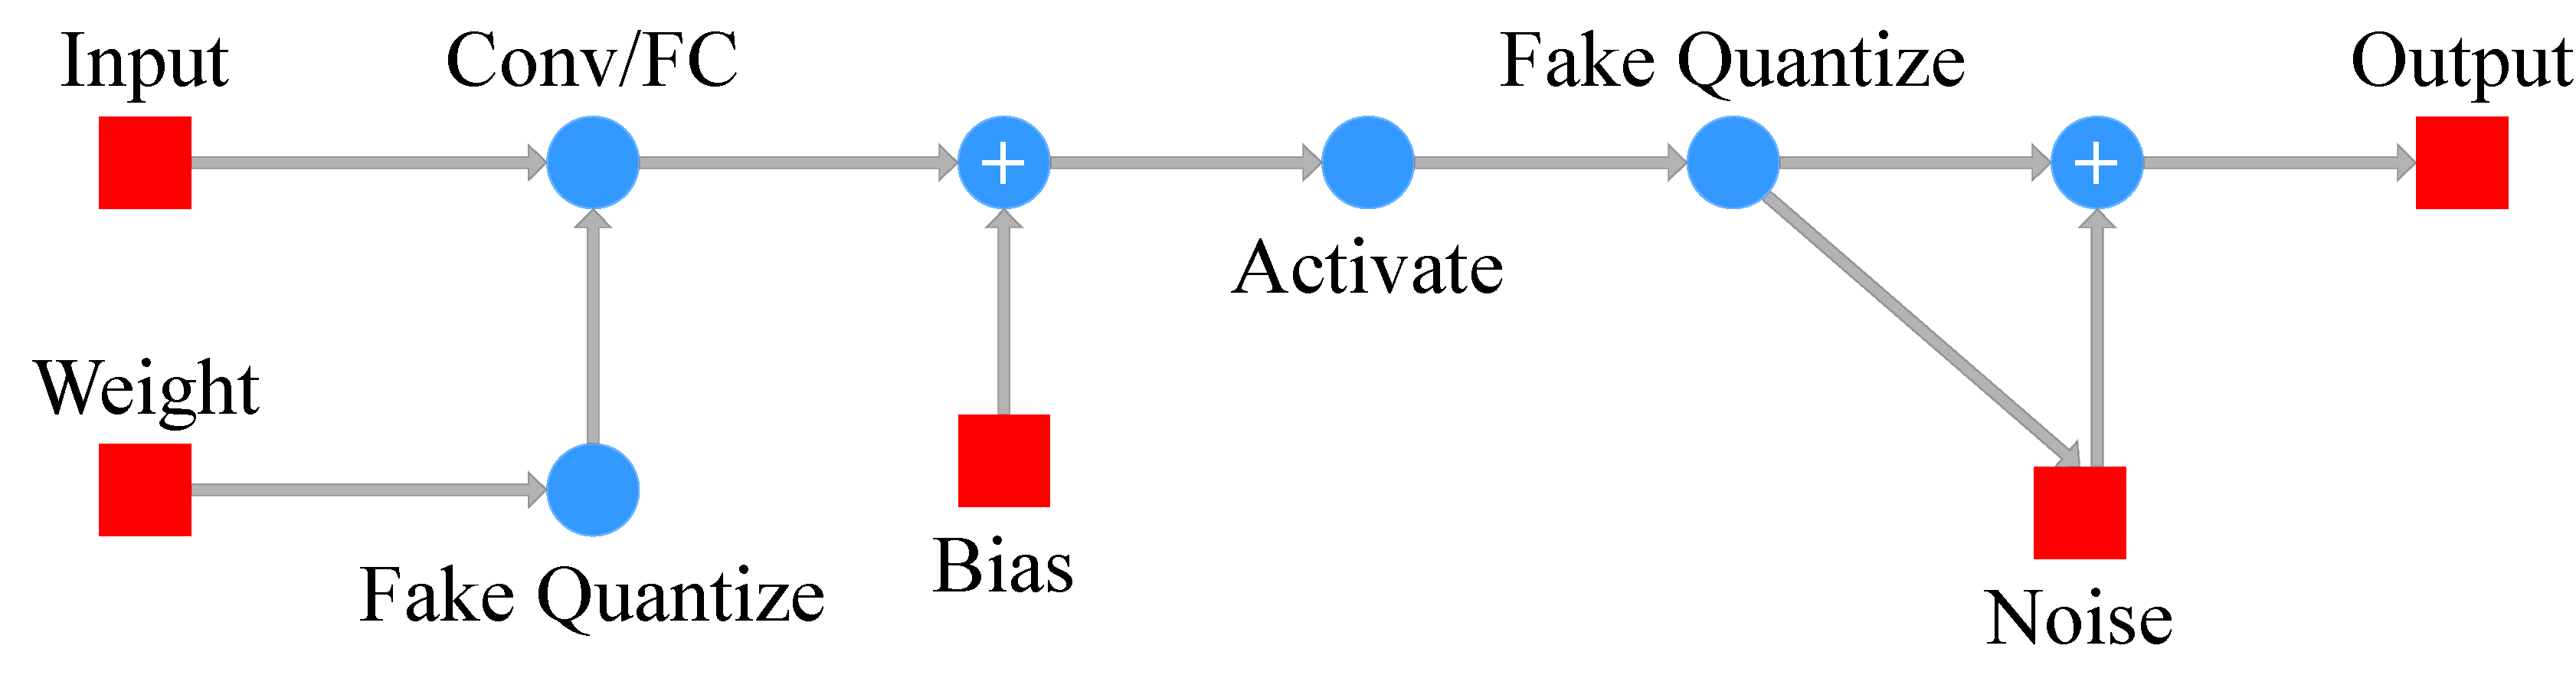
\includegraphics[width=0.85\linewidth]{./figs/DNN-ApproxFlow_fake_quantize.pdf}
    \caption{采用伪量化方法的基于噪声训练的DNN计算流图}
    \label{DNN:ApproxFlow:Fig:fake_quantize_noise}
\end{figure}

为了减少由于量化造成的精度损失,对DNN采用了伪量化方法\cite{DNN:fake_quanti},如图\ref{DNN:ApproxFlow:Fig:fake_quantize_noise}所示。伪量化操作应用于权重和激活函数(Activation function),由量化级别$t$和钳位范围$[a,b]$两个参数组成,通过逐点应用函数$q$来进行伪量化操作,$q$被定义为:
\begin{align}
    clamp(r, a, b) &= min(max(r, a), b) \\
    s(a, b, t)     &= \frac{b - a}{t - 1} \\
    q(r, a, b, t)  &= a + \lfloor \frac{clamp(r, a, b) - a}{s(a, b, t)} \rceil
\label{DNN:ApproxFlow:Eq:fake_quantize}
\end{align}
其中$r$表示要量化的实数,$\lfloor \ \rceil$表示四舍五入到最接近的整数。在8比特伪量化中,$n=2^8=256$,$a=min(r)$,$b=max(r)$。
对于批归一化(Batch Normalization, BN)的DNN,在伪量化过程开始时将每个BN层与其前一层合并,可在保持高精度的同时简化量化后的计算。合并操作可以通过以下等式来描述:
\begin{equation}
    \label{DNN:ApproxFlow:Eq:BN}
    \begin{aligned}
    \hat{w} = \frac{\gamma}{\sqrt{\sigma^2 + \epsilon}} w
    \end{aligned}
\end{equation}
其中$w$是原始权重张量,$\hat{w}$是合并后的权重张量,$\gamma$表示BN层的尺度参数,$\sigma ^2$表示激活方差,$\epsilon$是一个用于保持数值稳定性的常数。

另外,在伪量化\cite{DNN:fake_quanti}过程中,利用噪声训练(Noise training)技术来减少由于近似乘法器的引入造成的精度损失。图\ref{DNN:ApproxFlow:Fig:fake_quantize_noise}展示了带有噪声训练技术的DNN计算流图,其中输出是激活加上噪声,用于模拟近似乘法引起的计算误差,噪声$n(y)$根据激活$y$生成,$n(y)$被定义为:
\begin{equation}
    \label{DNN:ApproxFlow:Eq:noise}
    n(y) = \alpha \times rand(-1.0, 1.0) \times \vert y \vert
\end{equation}
其中$\alpha$表示噪声幅度,$rand(-1.0,1.0)$表示在$-1.0$到$1.0$之间随机取值。图~\ref{DNN:ApproxFlow:Fig:noise}显示了基于不同噪声幅值($\alpha \in \{0,0.2,0.4,0.6,0.8\}$)训练并近似后的AlexNet网络\cite{DNN:AlexNet}在CIFAR-10\cite{DNN:CIFAR-10}推理数据集上的精度,可以看到噪声幅度$\alpha > 0$时的精度比$\alpha = 0$时更高,这表明了噪声训练技术的有效性。同时,$\alpha$为0.8时AlexNet实现了最高的精度,在本文中,如果不特殊说明,所有DNN的噪声幅度$\alpha$取值均为$0.8$。
\begin{figure}[!ht]
    \centering
    \includegraphics[width=0.7\linewidth]{./figs/DNN-ApproxFlow_noise.pdf}
    \caption{不同噪声幅值训练并近似后的AlexNet神经网络在CIFAR-10推理数据集上的精度}
    \label{DNN:ApproxFlow:Fig:noise}
\end{figure}

\section{实验结果} \label{ASIC实验结果}

为了详细评估所提出的方法的有效性,对不同应用进行了实验,并与国际前沿工作进行比较,具体步骤如下:
首先确定乘法器的位宽,并提取输入数据分布,基于给定的面积减少比例$R$通过式\eqref{AC:AM:Adapt:Eq:l_approx}和算法\ref{AC:AM:Adapt:Alg:lambda}得到合适的$l$和$\lambda$的取值,然后根据式\eqref{AC:AM:Adapt:Eq:Obj}生成两个输入极性相反的优化目标函数(注意均匀分布下不需要考虑极性);
之后利用MATLAB混合整数遗传算法MIGA在一台拥有72核256GB内存的Intel Xeon服务器上分别对两个目标函数运行48小时进行求解,生成近似乘法器,挑出目标值最小的一批乘法器并与已有的工作进行比较。
比较的近似乘法器包括KMap\cite{AC:AM:KMap}、SDLC\cite{AC:AM:SDLC}、CR\cite{AC:AM:CR}、AC\cite{AC:AM:AC}、OU\cite{AC:AM:OU}、RoBA\cite{AC:AM:RoBA}、DRUM\cite{AC:AM:DRUM}、TOSAM\cite{AC:AM:TOSAM}、PPAM\cite{AC:AM:PPAM}。其中,SDLC采用2比特或门进行压缩,以实现最高的精度;CR的误差补偿模块通过6比特和7比特两种位宽进行实现,分别命名为C.6和C.7;OU原本是面向浮点数乘法器设计的,将其修改为定点数乘法器并使用1次划分和3次划分方式进行误差补偿,分别命名为L.1和L.3;DRUM的参数$m$分别取4,5,6,7进行实现;TOSAM中的可配置参数$h$和$t$取$\{0, 1, 2\} \times \{1, 2, 3\}$进行实现;PPAM中的可配置参数$i$和$j$取$\{0, 1, 2\} \times \{1, 2, 3\}$进行比较。同时,基于CGP方法生成的两个近似算术单元库Evoapprox8b(Evo8)\cite{AC:AM:CGP_Evoapprox8b}和EvoApproveLib$^\text{LITE}$(EvoLite)\cite{AC:AM:CGP_EvoLite}也参与评估。

所有乘法器的精度均由应用的精度表示,注意对于没有标明输入的非对称乘法器在交换输入后也有一个精度,为保证公平,取最高的精度参与比较;硬件指标包括面积、延迟、功耗,均在一定的时钟频率约束下由Synopsys Design Compiler (DC) S-2021.06-SP5基于一个开源的7nm工艺库\cite{ASAP7_github}综合得到。对精确乘法器来讲,DC会调用DesignWare库\cite{IP:DesignWare}进行实现,实现的精确乘法器被称为DesignW。


\subsection{均匀分布下的8比特无符号乘法器}

假设某一应用中乘法器的输入为8比特无符号数,且数据是均匀分布的(无需考虑输入极性),应用精度是乘法器的平均绝对误差MAE(即平均误差距离MED,见式\eqref{AC:Arith:MED})。

\begin{figure}[!h]
    \centering
    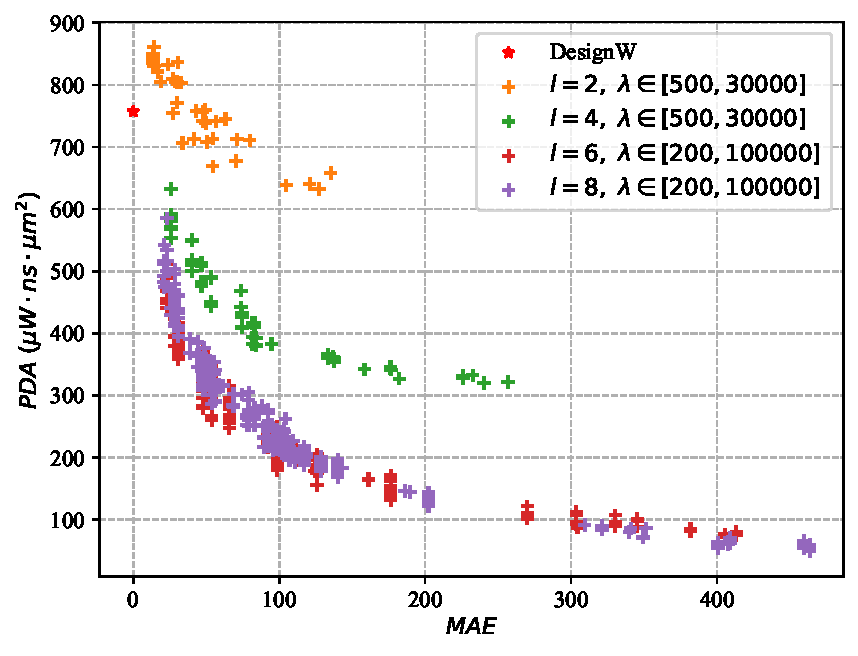
\includegraphics[width=0.8\linewidth]{figs/AC-AM-Adapt-uniform_8x8_diff_l.pdf}
    \caption{不同$l$和$\lambda$取值下生成的近似乘法器的MAE和PDA散点图比较}
    \label{AC:AM:Adapt:Fig:uniform_8x8_diff_l}
\end{figure}

为方便比较,忽略$R$,直接对$l$取2,4,6,8并对$\lambda$进行不同取值的尝试,生成的乘法器的MAE和PDA散点图如图\ref{AC:AM:Adapt:Fig:uniform_8x8_diff_l}所示,其中PDA是在2GHz的时钟频率约束下得到的,DesignW代表精确乘法器,可以看到$l$的取值决定了近似乘法器PDA的提升上限($l=6$、8时区分不太明显),$l$和$\lambda$越大,生成的乘法器的硬件开销越小,但代价是误差较大。

\begin{figure}[!h]
    \centering
    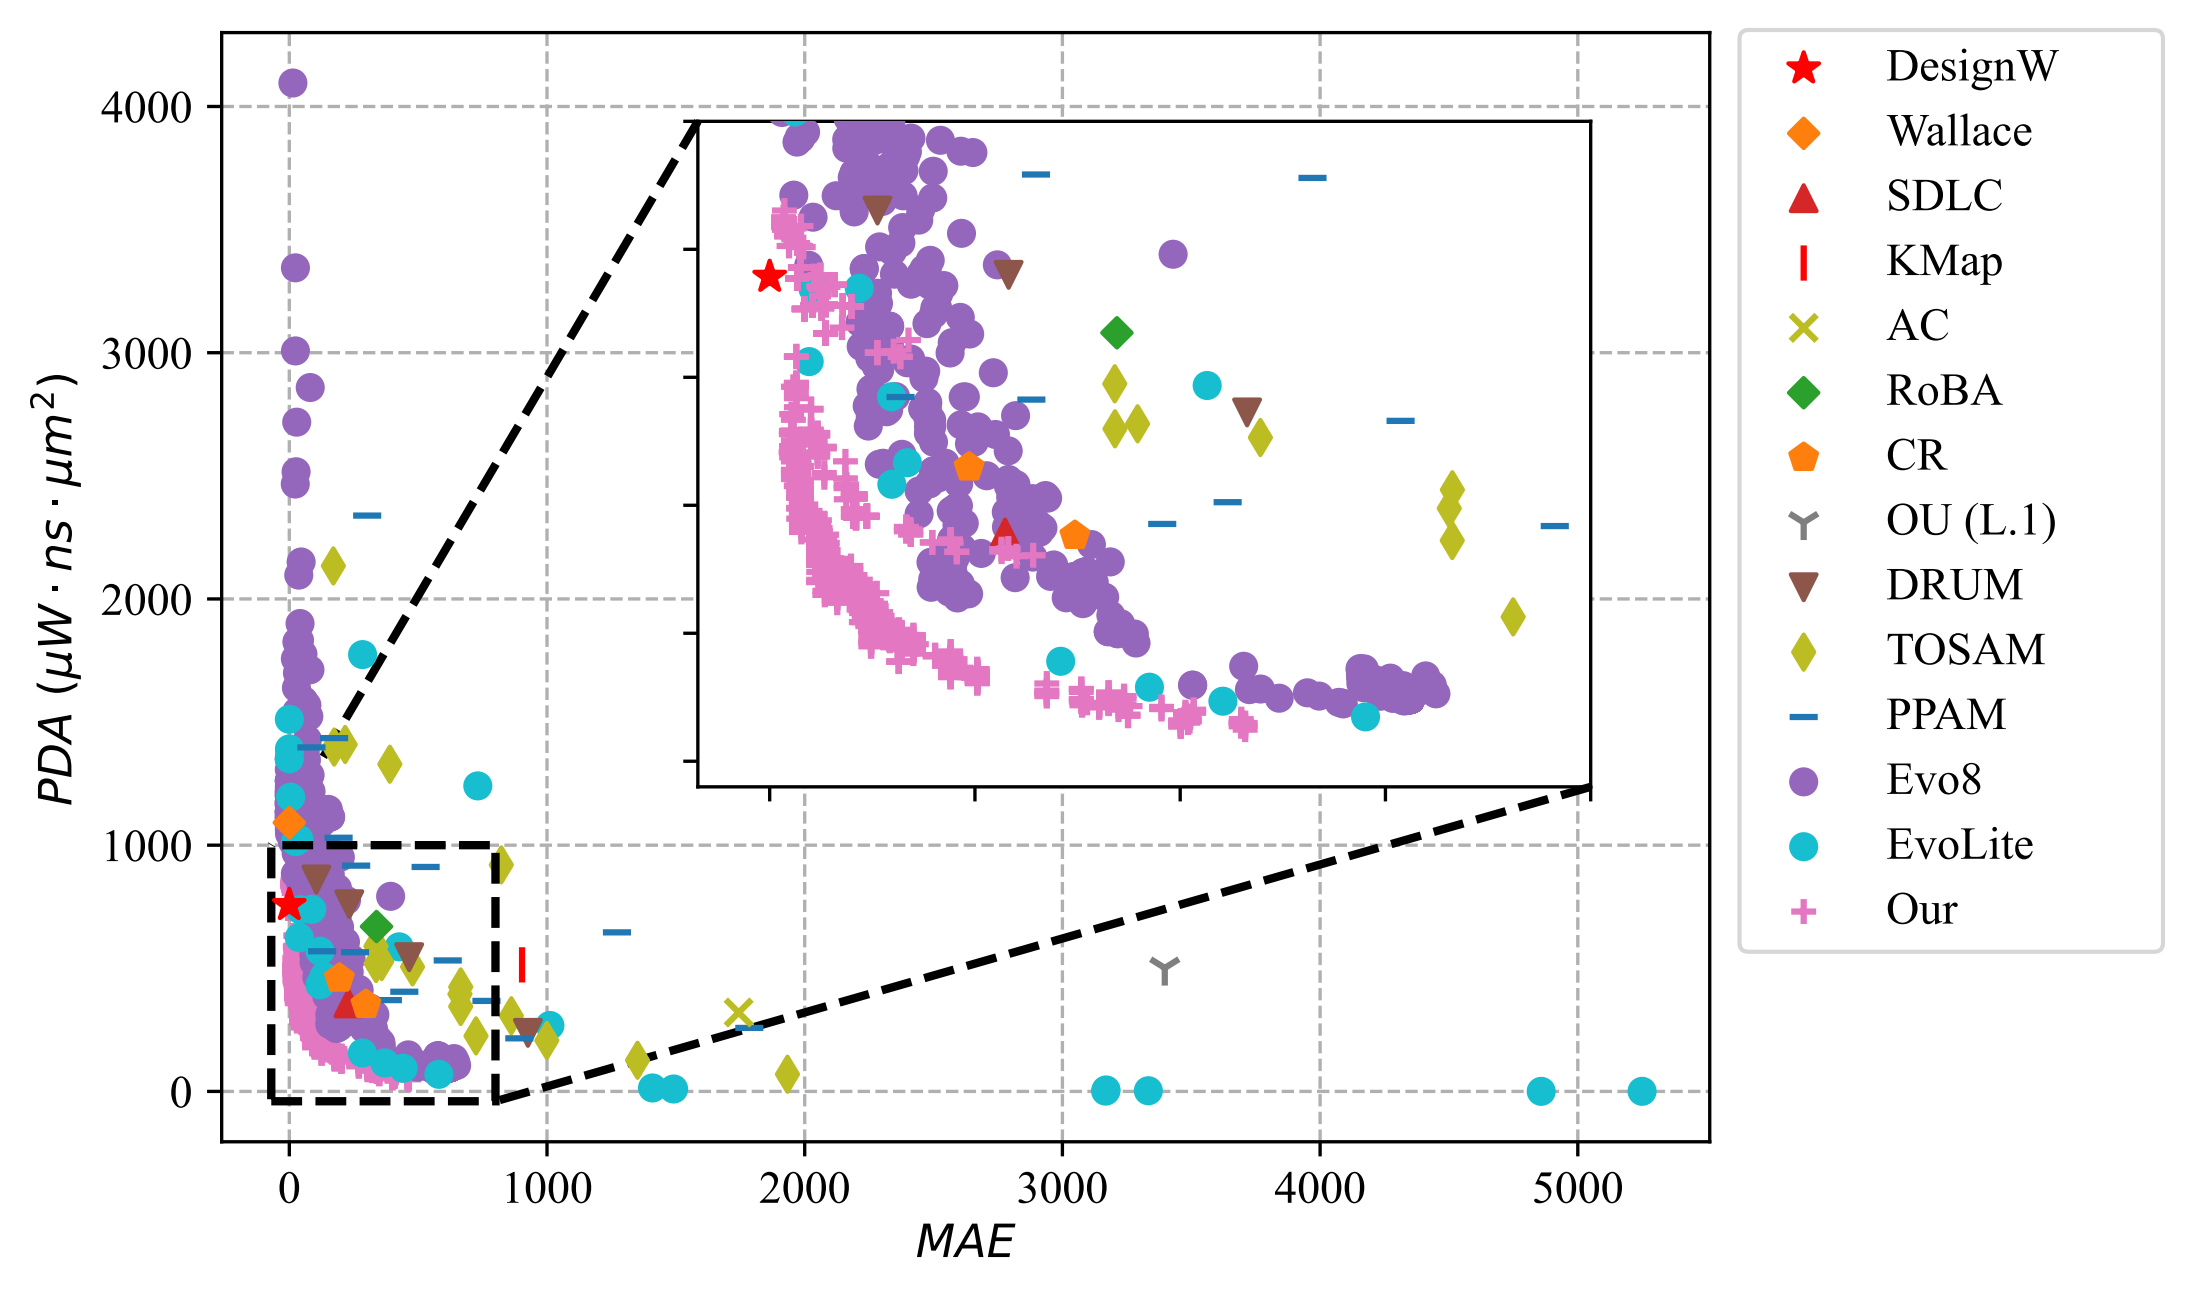
\includegraphics[width=\linewidth]{figs/AC-AM-Adapt-uniform_8x8_PDA_MAE.png}
    \caption{生成的近似乘法器与国际前沿工作进行MAE和PDA比较}
    \label{AC:AM:Adapt:Fig:uniform_8x8_PDA_MAE}
\end{figure}
图\ref{AC:AM:Adapt:Fig:uniform_8x8_PDA_MAE}展示了生成的近似乘法器与国际前沿工作进行PDA和MAE对比的散点图,时钟频率约束为2GHz。在该图中,越靠近左下角的乘法器质量越好,可以看到本文提出的基于多种操作对部分积进行压缩的自动化方法取得了显著的优势,在MAE和PDA两方面都领先于绝大部分已有的近似乘法器。
% 未来可能也很难有比本文效果更好的方法出现。
最后,从图\ref{AC:AM:Adapt:Fig:uniform_8x8_PDA_MAE}中可以看到DesignW的PDA比许多近似乘法器都要好,这表明在设计近似乘法器时应当想办法充分利用EDA工具本身所具有的优势。


\subsection{基于8比特无符号数的不同规模的DNN应用}

从DNN中提取乘法器的输入分布,并在某个特定的$R$下按照如前所述的方法生成近似乘法器,之后与已有的近似乘法器一起在考虑极性的情况下利用提出的DNN推断精度评估工具对近似后的神经网络进行精度评估,并利用DC进行综合以比较硬件性能。DNN中乘法器的两个操作数分别是特征输入(Feature input)和权重(Weight),两者的概率分布通常不同,因此按照本文提出的方法对DNN生成近似乘法器时需考虑极性,设XFYW代表$P=0$的乘法器($x$是特征输入、$y$是权重),XWYF代表$P=1$的乘法器($x$是权重、$y$是特征输入)。

为了对不同乘法器的质量进行统一比较,引入功耗、延迟、面积、相对精度损失4个指标的乘积(Product of relative accuracy loss and PDA, APDA)来衡量不同乘法器在某个DNN应用中的好坏,相对精度损失定义为:
\begin{equation}
     \text{ceil}_\% ( A_{exact} ) - A_{mul}
\label{AC:AM:Adapt:LeNet:Eq:accuracy_loss}
\end{equation}
式中$A_{exact}$表示DNN在精确乘法器下的精度,$\text{ceil}_\%()$表示百分比格式的向上取整,如$\text{ceil}_\%(88.39\%) = 89\% $,$A_{mul}$表示DNN在某个乘法器下的精度,注意精确乘法器的相对精度损失可能不为0。

\subsubsection{LeNet和MNIST}

\begin{figure}[!h]
    \centering
    \subfigure[输入数据直方图]{
    \label{DNN:LeNet:Fig:LeNet_MNIST_input}
    \begin{minipage}[t]{0.48\linewidth}
    \centering
    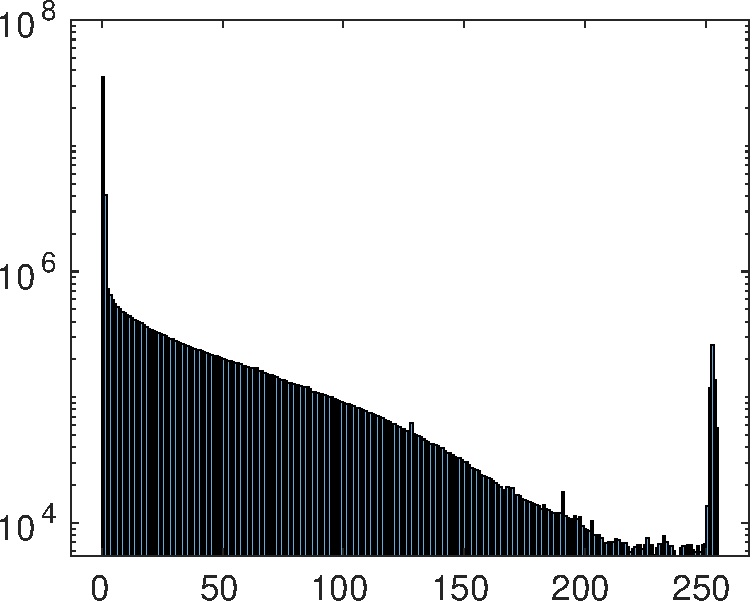
\includegraphics[width=\linewidth]{./figs/DNN-LeNet_MNIST_input.pdf}
    \end{minipage}
    }%
    \subfigure[权重数据直方图]{
    \label{DNN:LeNet:Fig:LeNet_MNIST_weight}
    \begin{minipage}[t]{0.48\linewidth}
    \centering
    \includegraphics[width=\linewidth]{./figs/DNN-LeNet_MNIST_weight.pdf}
    \end{minipage}
    }
    \centering
    \caption{基于8比特无符号数量化的LeNet网络在MNIST推理数据集上的输入和权重数据直方图}
    \label{DNN:LeNet:Fig:LeNet_MNIST_distribution}
\end{figure}

\begin{table*}[ht]
    \renewcommand{\arraystretch}{1.3}
    \setlength\tabcolsep{3.76pt}
    \caption{采用不同近似乘法器近似后的LeNet网络在MNIST数据集的精度}
    \label{AC:AM:Adapt:LeNet:Table:accuracies}
    \centering
    \scalebox{0.585}{
    \begin{tabular}{|c|c|c|c|c|c|c|c|c|c|c|c|c|c||c|}
      \hline
      \multirow{2}{*}{\textbf{Metric}} & \textbf{KMap} & \textbf{CR (C.6)} & \textbf{CR (C.7)} & \textbf{AC} & \textbf{RoBA} & \textbf{OU (L.1)} & \textbf{OU (L.3)} & \textbf{SDLC} & \textbf{DRUM} & \textbf{TOSAM} & \textbf{PPAM} & \textbf{Evo8} & \textbf{EvoLite} & \multirow{2}{*}{\textbf{Exact}} \\
      & \cite{AC:AM:KMap} & \cite{AC:AM:CR} & \cite{AC:AM:CR} & \cite{AC:AM:AC} & \cite{AC:AM:RoBA} & \cite{AC:AM:OU} & \cite{AC:AM:OU} & \cite{AC:AM:SDLC} & \cite{AC:AM:DRUM} & \cite{AC:AM:TOSAM} & \cite{AC:AM:PPAM} & \cite{AC:AM:CGP_Evoapprox8b} & \cite{AC:AM:CGP_EvoLite} & \\
      \hline
      \multirow{2}{*}{Accuracy (\%)} & \multirow{2}{*}{96.32} & 74.88 /  & 97.77 /  & \multirow{2}{*}{18.28} & \multirow{2}{*}{\textbf{99.31}} & \multirow{2}{*}{11.35} & \multirow{2}{*}{97.28} & \textbf{98.07 / } & 26.01 -  & 19.72 -  & 9.8 -  & 9.74 -  & 9.78 -  & \multirow{2}{*}{\textbf{99.41}} \\
      &  & 81.79 & \textbf{98.26} &  &  &  &  & 97.92 & 99.1 & 99.32 & 99.27 & 99.43 & 99.42 & \\
      \hline
    \end{tabular}
    }
\end{table*}

首先对基于8比特无符号数量化的LeNet网络在MNIST推理数据集\cite{DNN:LeNet_MNIST}上的数据进行分析,提取了所有层的输入和权重数据,直方图分别如图\ref{DNN:LeNet:Fig:LeNet_MNIST_input}和图\ref{DNN:LeNet:Fig:LeNet_MNIST_weight}所示,可以看到输入集中在0和255附近,权重集中在128附近。
设$R=0.4$,由式\eqref{AC:AM:Adapt:Eq:l_approx}得$l$为6,即选择8$\times$8无符号乘法器的前6行部分积进行分簇压缩,且需要考虑输入极性。由算法\ref{AC:AM:Adapt:Alg:lambda}得$P=0$和$P=1$时的$\lambda$均为5000,与$l=6$一起根据式\eqref{AC:AM:Adapt:Eq:Obj}生成近似乘法器。

表\ref{AC:AM:Adapt:LeNet:Table:accuracies}展示了在考虑输入极性的情况下采用不同近似乘法器近似后的LeNet网络在MNIST数据集的精度,KMap、AC、RoBA、OU、DRUM、TOSAM、以及Evo8和EvoLite中的一些乘法器是对称的。
Evo8中的三个乘法器mul8\_98、mul8\_108和mul8\_154的精度最高,达到99.43\%,但它们的硬件性能太差,例如,在2GHz的时钟频率约束下,mul8\_108的PDA是DesignW的2倍。在EvoLite中,mul8u\_ZFB精度最高,为99.39\%。
为了直观地看出不同乘法器的质量高低,选择表\ref{AC:AM:Adapt:LeNet:Table:accuracies}精度高于98\%的乘法器(Evo8中精度高于99.2\%的乘法器)与生成的乘法器进行比较,结果如图\ref{AC:AM:Adapt:Fig:LeNet_PDA_accuracy}所示,PDA是基于2GHz的时钟频率约束下得到的,XFYW和XWYF分别代表基于$P=0$和$P=1$生成的近似乘法器。

\begin{figure}[!h]
    \centering
    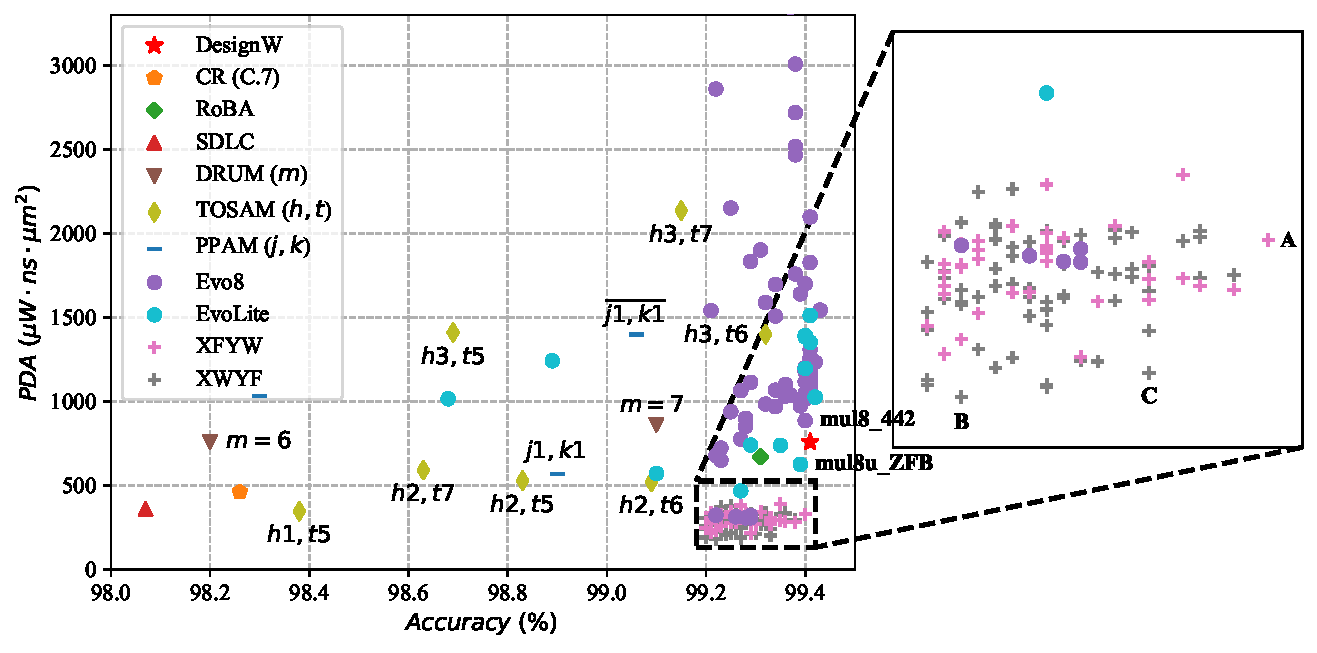
\includegraphics[width=\linewidth]{figs/AC-AM-Adapt-LeNet_PDA_accuracy.pdf}
    \caption{不同乘法器在LeNet和MNIST上的精度以及2GHz时钟频率约束下的PDA散点图}
    \label{AC:AM:Adapt:Fig:LeNet_PDA_accuracy}
\end{figure}

在图\ref{AC:AM:Adapt:Fig:LeNet_PDA_accuracy}中,PPAM($\overline{j,k}$)表示PPAM($j,k$)的比较器版本,该版本通过引入一个比较器决定是否交换乘法器的两个输入来提高乘法器的精度。从图中可以看到,TOSAM的效果好于DRUM,这是合理的,因为TOSAM有一个额外的截断操作来减少误差。对于PPAM来说,同样配置参数下有比较器的版本精度更高,但代价是消耗了更多的硬件资源。
基于本文的方法生成的乘法器XFYW和XWYF中,\emph{`A'}、\emph{`B'}和\emph{`C'}分别代表了精度最高、硬件成本最低、以及精度硬件权衡最好的三个乘法器。乘法器\emph{`A'}的精度为99.4\%,仅比精确乘法器的精度低0.01\%。与DesignW、Evo8中的mul8\_442、EvoLite中的mul8u\_ZFB和TOSAM(3,6)相比,\emph{`A'}的PDA分别提升了56.8\%、63.0\%、47.6\%和76.6\%。
\emph{`B'}以小于0.2\%的精度损失实现了图\ref{AC:AM:Adapt:Fig:LeNet_PDA_accuracy}所有的乘法器中最低的PDA值,与SDLC、DRUM(6)和TOSAM(1,5)相比,\emph{`B'}的PDA分别改善了50.3\%、76.6\%和48.4\%。
与RoBA相比,乘法器\emph{`C'}的精度高了0.02\%,PDA低了70.0\%。
极性相反的XFYW和XWYF乘法器并没有表现出明显的质量区别,这可能是由于LeNet网络结构简单、对误差的容忍性较大的原因。

\begin{figure}[!h]
    \centering
    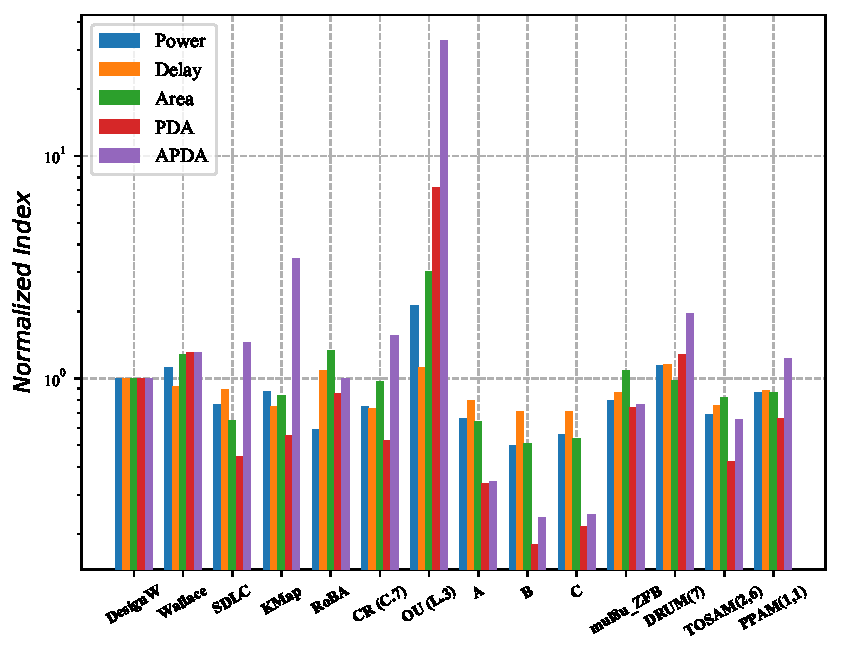
\includegraphics[width=0.9\linewidth]{figs/AC-AM-Adapt-LeNet_hist.pdf}
    \caption{基于LeNet和MNIST的不同乘法器的功耗、延迟、面积、PDA和APDA,以DesignW为标准进行归一化}
    \label{AC:AM:Adapt:Fig:LeNet_hist}
\end{figure}

图\ref{AC:AM:Adapt:Fig:LeNet_hist}展示了以DesignW为标准进行归一化后的不同近似乘法器的功耗、延迟、面积、PDA和APDA,数据基于0.5GHz的时钟频率约束得到,其中Wallace是采用华莱士树方法(见\ref{华莱士树})对部分积进行累加的乘法器。
可以看到,RoBA是一种以面积换取功耗的设计;OU的电路面积随着误差补偿级别的提高增长过快;CR乘法器的延迟极低,这符合它仅允许进位信号最多传播两个全加器的设计理念;EvoLite中的mul8u\_ZFB乘法器的面积略大于DesignW,这表示基于门级结构对精确乘法器进行简化效率不高;
DRUM(7)的功耗和延迟都略高于DesignW,这是因为需要检查的比特数为7,检测器的成本超过了小位宽乘法器带来的受益;TOSAM(2,6)的APDA比PDA高出一大截,这表明其硬件开销低,但精度损失稍大。
同时可以观察到,乘法器\emph{`A'}、\emph{`B'}、\emph{`C'}在功耗、延迟、面积、PDA和APDA方面优于所有乘法器。与mul8u\_ZFB相比,\emph{`A'}的面积减少了44.57\%,延迟减少了6.3\%,功耗减少了13.14\%,PDA减少了54.4\%,APDA减少了55.1\%。与RoBA相比,\emph{`C'}在面积、延迟和功耗方面分别提升了59.6\%、34.0\%、5.1\%、60.3\%和65.5\%。

\begin{figure}[!ht]
    \centering
    \subfigure{
      \label{AC:AM:Adapt:Fig:Acc_legend}
      \begin{minipage}[t]{0.95\linewidth}
        \centering
        \includegraphics[width=\linewidth]{./figs/AC-AM-Adapt-Accs_legend.pdf}
      \end{minipage}
    }
    \setcounter{subfigure}{0}
    \subfigure[1GHz、1.5GHz和2GHz下的SA]{
      \label{AC:AM:Adapt:Fig:Acc_SA}
      \begin{minipage}[t]{0.33\linewidth}
        \centering
        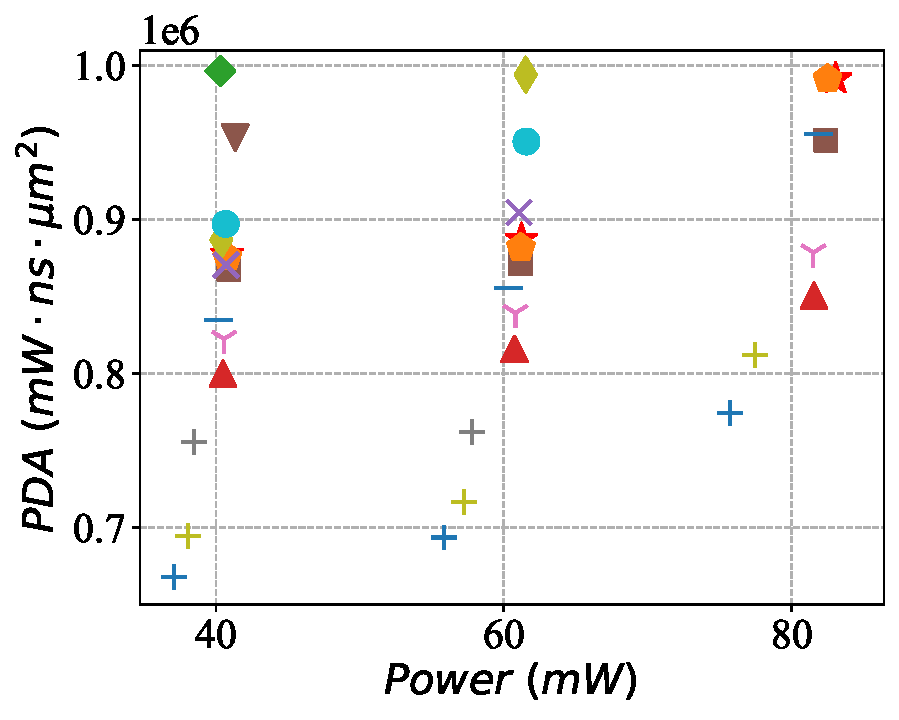
\includegraphics[width=\linewidth]{./figs/AC-AM-Adapt-Acc_SA.pdf}
      \end{minipage}
    }%
    \subfigure[1.5GHz、2GHz和2.5GHz的SC]{
      \label{AC:AM:Adapt:Fig:Acc_SC}
      \begin{minipage}[t]{0.33\linewidth}
        \centering
        \includegraphics[width=\linewidth]{./figs/AC-AM-Adapt-Acc_SC.pdf}
      \end{minipage}
      \hspace{-4.3mm}
    }%
    \subfigure[1GHz和1.5GHz下的TASU]{
      \label{AC:AM:Adapt:Fig:Acc_TASU}
      \begin{minipage}[t]{0.33\linewidth}
        \centering
        \includegraphics[width=\linewidth]{./figs/AC-AM-Adapt-Acc_TASU.pdf}
      \end{minipage}
      \hspace{-4.7mm}
    }%
    \centering
    \caption{不同DNN加速器在多个时钟频率约束下基于不同乘法器得到的功耗和PDA指标}
    \label{AC:AM:Adapt:Fig:Accs}
\end{figure}

为了展示近似乘法器对实际的DNN硬件加速器到底带来了多少收益,将不同的近似乘法器对三个DNN加速器中的精确乘法器进行替换并利用DC进行综合得到功耗、延迟和面积,考虑的加速器包括:(1)针对DoReFa-Net网络\cite{DNN:DoReFa-Net}设计的TASU\cite{Accelerator:JiaoLi};(2)针对DNN中卷积操作进行加速的SC\cite{Accelerator:SC};(3)谷歌的TPU采用的脉动阵列(Systolic Array)架构\cite{Accelerator:TPU},简称为SA。

图\ref{AC:AM:Adapt:Fig:Accs}展示了三个加速器基于不同近似乘法器在多个时钟频率约束下得到的功耗和PDA指标,其中SA的规模为16$\times$16。可以看到,基于\emph{`B'}和\emph{`C'}的实现的SA和SC在实验的所有频率下都优于基于其他乘法器实现的版本。
基于PPAM(1,1)的TASU加速器功耗和PDA较低,这可能是因为PPAM在Verilog编写时采用多位宽的“+”运算符来对乘法器的部分积进行累加,能够让EDA工具对其进行有效地优化。

\subsubsection{AleNet和CIFAR-10}

\begin{figure}[!h]
    \centering
    \subfigure[输入数据直方图]{
    \label{DNN:LeNet:Fig:AlexNet_CIFAR-10_input}
    \begin{minipage}[t]{0.48\linewidth}
    \centering
    \includegraphics[width=\linewidth]{./figs/DNN-AlexNet_CIFAR-10_input.pdf}
    \end{minipage}
    }%
    \subfigure[权重数据直方图]{
    \label{DNN:LeNet:Fig:AlexNet_CIFAR-10_weight}
    \begin{minipage}[t]{0.48\linewidth}
    \centering
    \includegraphics[width=\linewidth]{./figs/DNN-AlexNet_CIFAR-10_weight.pdf}
    \end{minipage}
    }
    \centering
    \caption{基于8比特位宽量化的AlexNet网络在CIFAR-10推理数据集上的输入和权重数据直方图}
    \label{DNN:LeNet:Fig:AlexNet_CIFAR-10_distribution}
\end{figure}


为了验证提出的方法对不同规模神经网络的有效性,对基于CIFAR-10数据集\cite{DNN:CIFAR-10}的AlexNet网络\cite{DNN:AlexNet}进行了类似的实验,从AlexNet中提取的输入和权重数据直方图如图\ref{DNN:LeNet:Fig:AlexNet_CIFAR-10_distribution}所示,可以看到其概率分布与基于MNIST的LeNet网络类似\cite{DNN:LeNet_MNIST},但数据的集中程度更高。
与LeNet相比,AlexNet的网络深度更大,在采用相同近似乘法器时会导致更大的累积误差,引起更多的精度下降。考虑到AlexNet对误差的容忍性不如LeNet,假设$R=0.3$,由式\eqref{AC:AM:Adapt:Eq:l_approx}得$l=4$,即取8$\times$8无符号乘法器的前四行部分积进行压缩,同时由算法\ref{AC:AM:Adapt:Alg:lambda}得$P=0$和$P=1$时的$\lambda$均为500,与$l=4$一起根据式\eqref{AC:AM:Adapt:Eq:Obj}生成近似乘法器。

\begin{table*}
    \renewcommand{\arraystretch}{1.3}
    \setlength\tabcolsep{3.76pt}
    \caption{采用不同近似乘法器近似后的AlexNet网络在CIFAR-10数据集的精度}
    \label{AC:AM:Adapt:AlexNet:Table:accuracies}
    \centering
    \scalebox{0.585}{
    \begin{tabular}{|c|c|c|c|c|c|c|c|c|c|c|c|c|c||c|}
      \hline
      \multirow{2}{*}{\textbf{Metric}} & \textbf{KMap} & \textbf{CR (C.6)} & \textbf{CR (C.7)} & \textbf{AC} & \textbf{RoBA} & \textbf{OU (L.1)} & \textbf{OU (L.3)} & \textbf{SDLC} & \textbf{DRUM} & \textbf{TOSAM} & \textbf{PPAM} & \textbf{Evo8} & \textbf{EvoLite} & \multirow{2}{*}{\textbf{Exact}} \\
      & \cite{AC:AM:KMap} & \cite{AC:AM:CR} & \cite{AC:AM:CR} & \cite{AC:AM:AC} & \cite{AC:AM:RoBA} & \cite{AC:AM:OU} & \cite{AC:AM:OU} & \cite{AC:AM:SDLC} & \cite{AC:AM:DRUM} & \cite{AC:AM:TOSAM} & \cite{AC:AM:PPAM} & \cite{AC:AM:CGP_Evoapprox8b} & \cite{AC:AM:CGP_EvoLite} & \\
      \hline
      \multirow{2}{*}{Accuracy (\%)} & \multirow{2}{*}{49.67} & 10 /  & 10.01 /  & \multirow{2}{*}{10.06} & \multirow{2}{*}{8.92} & \multirow{2}{*}{10} & \multirow{2}{*}{61.21} & 10.29 /  & 10.0 -  & 9.09 -  & 10.0 -  & 9.85 -  & 10.0 -  & \multirow{2}{*}{\textbf{88.39}} \\
      &  & 10 & 10.02 &  &  &  &  & 24.94 & 87.5 & 86.81 & 85.86 & 88.54 & 88.47 & \\
      \hline
    \end{tabular}
    }
\end{table*}


表\ref{AC:AM:Adapt:AlexNet:Table:accuracies}展示了在考虑输入极性的情况下采用不同近似乘法器近似后的AlexNet网络在CIFAR-10数据集的精度,可以看到与LeNet相比下降了很多。
在表\ref{AC:AM:Adapt:AlexNet:Table:accuracies}中,OU(L.3)的精度远高于KMap、RoBA和SDLC,这主要是因为OU(L.3)采用了3次划分的设计方式,提供了足够的误差补偿。DRUM(7)、TOSAM(3,5)、PPAM(0,1)和PPAM($\overline{0,1}$)精度分别为87.50\%、86.81\%、85.63\%和85.86\%,但它们的在2GHz下的PDA平均比DesignW多了18.5\%。

\begin{figure}[!htb]
    \centering
    \includegraphics[width=0.9\linewidth]{figs/AC-AM-Adapt-AlexNet_CIFAR-10_PDA_accuracy.pdf}
    \caption{不同乘法器在AlexNet和CIFAR-10上的精度以及2GHz时钟频率下的PDA散点图}
    \label{AC:AM:Adapt:Fig:AlexNet_CIFAR-10_PDA_accuracy}
\end{figure}

图\ref{AC:AM:Adapt:Fig:AlexNet_CIFAR-10_PDA_accuracy}展示了不同乘法器基于CIFAR-10\cite{DNN:CIFAR-10}数据集和ALexNet网络\cite{DNN:AlexNet}得到的精度,以及利用DC在2GHz时钟频率约束下获得的PDA散点图,为了保证公平,除了标明输入的XFYW和XWYF之外,其余所有的非对称乘法器都是取$P=0$和$P=1$下精度较高的值参与比较。图\ref{AC:AM:Adapt:Fig:AlexNet_CIFAR-10_PDA_accuracy}只显示了一部分乘法器的原因是只有这部分乘法器的精度和PDA在坐标表示的范围之内,其余的乘法器要么精度不够、要么PDA太差。对比的精确乘法器有两个版本,分别是DesignW和Wallce。
可以看到,虽然Evo8中有些乘法器的精度很高,但PDA比DesignW和Wallace还要差,硬件成本不可接受。EvoLite中的mul8u\_ZFB乘法器以精度损失小于$0.1\%$的代价实现了比DesignW更好的PDA值,是一个不错的设计。

值得一提的是,基于本文的方法生成的近似乘法器XFYW和XWYF效果最好,由于DNN的特性,甚至存在近似后神经网络的精度更高的情况,这可能是因为DNN的冗余性。
如图\ref{AC:AM:Adapt:Fig:AlexNet_CIFAR-10_PDA_accuracy}中的乘法器$\emph{`E'}$、$\emph{`D'}$、$\emph{`F'}$所示,它们不仅拥有比DesignW更低的PDA,还拥有比DesignW更高的精度。
另一个有趣的现象是,基于$P=0$生成的XFYW乘法器的精度普遍比基于$P=1$生成的XWYF乘法器的精度要高,这有力地证明了在设计近似乘法器时考虑输入极性的重要性。
在所有生成的乘法器中,$\emph{`G'}$的PDA最低,与DesignW和mul8u\_ZFB相比,$\emph{`G'}$的PDA分别改进了45.8\%和34.3\%。选择6个生成的乘法器$\emph{`D'}$、$\emph{`E'}$、$\emph{`F'}$、$\emph{`G'}$、$\emph{`H'}$、$\emph{`I'}$与两个精确乘法器DesignW、Wallace和三个近似乘法器mul8u\_ZFB、DRUM(7)、TOSAM(3,5)进行进一步地比较。

\begin{figure}[!htb]
    \centering
    \includegraphics[width=0.9\linewidth]{figs/AC-AM-Adapt-AlexNet_CIFAR-10_hist.pdf}
    \caption{基于AlexNet和CIFAR-10的不同乘法器的功耗、延迟、面积、PDA和APDA,以DesignW为标准进行归一化}
    \label{AC:AM:Adapt:Fig:ALexNet_CIFAR-10_hist}
\end{figure}

图\ref{AC:AM:Adapt:Fig:ALexNet_CIFAR-10_hist}展示了11个乘法器在2GHz时钟频率约束下以DesignW为标准进行归一化后的功耗、延迟、面积、PDA和APDA比较图,
可以看到根据本文方法生成的6个乘法器拥有最优的PDA和APDA。TOSAM(3,5)的硬件成本过高,且精度损失也较大。
与DesignW相比,6个生成的乘法器($\emph{`D'} \sim \emph{`I'}$)平均改进了30.2\%的功耗、12.8\%的面积、38.4\%的PDA和36.8\%的APDA;
与mul8u\_ZFB相比,6个生成的乘法器平均改进了13.9\%的功耗、13.3\%的面积、25.3\%的PDA和31.3\%的APDA。

将基于AlexNet和CIFAR-10生成的乘法器(图\ref{AC:AM:Adapt:Fig:AlexNet_CIFAR-10_PDA_accuracy}中的XFYW和XWYF)放在LeNet和MNIST中进行评估,大部分乘法器的精度都在99\%以上,这表明按照本文的方法基于较大规模DNN生成的近似乘法器在面对较小规模DNN时表现出了一定的可迁移性。


\subsubsection{VGG16和CIFAR-10}

\begin{figure}[!h]
    \centering
    \subfigure[输入数据直方图]{
    \label{DNN:LeNet:Fig:VGG16_CIFAR-10_input}
    \begin{minipage}[t]{0.48\linewidth}
    \centering
    \includegraphics[width=\linewidth]{./figs/DNN-VGG16_CIFAR-10_input.pdf}
    \end{minipage}
    }%
    \subfigure[权重数据直方图]{
    \label{DNN:LeNet:Fig:VGG16_CIFAR-10_weight}
    \begin{minipage}[t]{0.48\linewidth}
    \centering
    \includegraphics[width=\linewidth]{./figs/DNN-VGG16_CIFAR-10_weight.pdf}
    \end{minipage}
    }
    \centering
    \caption{基于8比特位宽量化的VGG16网络在CIFAR-10推理数据集上的输入和权重数据直方图}
    \label{DNN:LeNet:Fig:VGG16_CIFAR-10_distribution}
\end{figure}

为了进一步证明提出的自动化近似乘法器设计方法在大规模神经网络下的适用性,对基于CIFAR-10数据集\cite{DNN:CIFAR-10}的VGG16神经网络\cite{DNN:VGG16}进行输入和权重的数据提取,直方图如图\ref{DNN:LeNet:Fig:VGG16_CIFAR-10_distribution}所示,可以看到其分布与LeNet和AlexNet相似。考虑到VGG16的网络层数比LeNet和AlexNet都大,
近似后的误差累计更多,能够在VGG16上不引起大幅精度下降的近似乘法器可能与精确乘法器相比没有特别明显的硬件优势,假设$R=0.2$,由式\eqref{AC:AM:Adapt:Eq:l_approx}得$l=4$,根据算法\ref{AC:AM:Adapt:Alg:lambda}得$P=0$和$P=1$时$\lambda=5000$,这里对$\lambda$进行调整,同时考虑$\lambda \in \{1000,2000,3000,4000,5000\}$生成近似乘法器。
\begin{table*}[ht]
    \renewcommand{\arraystretch}{1.3}
    \setlength\tabcolsep{3.76pt}
    \caption{采用不同近似乘法器近似后的VGG16网络在CIFAR-10数据集的精度}
    \label{AC:AM:Adapt:VGG16:Table:accuracies}
    \centering
    \scalebox{0.585}{
    \begin{tabular}{|c|c|c|c|c|c|c|c|c|c|c|c|c|c||c|}
      \hline
      \multirow{2}{*}{\textbf{Metric}} & \textbf{KMap} & \textbf{CR (C.6)} & \textbf{CR (C.7)} & \textbf{AC} & \textbf{RoBA} & \textbf{OU (L.1)} & \textbf{OU (L.3)} & \textbf{SDLC} & \textbf{DRUM} & \textbf{TOSAM} & \textbf{PPAM} & \textbf{Evo8} & \textbf{EvoLite} & \multirow{2}{*}{\textbf{Exact}} \\
      & \cite{AC:AM:KMap} & \cite{AC:AM:CR} & \cite{AC:AM:CR} & \cite{AC:AM:AC} & \cite{AC:AM:RoBA} & \cite{AC:AM:OU} & \cite{AC:AM:OU} & \cite{AC:AM:SDLC} & \cite{AC:AM:DRUM} & \cite{AC:AM:TOSAM} & \cite{AC:AM:PPAM} & \cite{AC:AM:CGP_Evoapprox8b} & \cite{AC:AM:CGP_EvoLite} & \\
      \hline
      \multirow{2}{*}{Accuracy (\%)} & \multirow{2}{*}{10} & 10.83 /  & 9.56 /  & \multirow{2}{*}{10.28} & \multirow{2}{*}{10.01} & \multirow{2}{*}{10.01} & \multirow{2}{*}{10} & 9.95 /  & 8.89 -  & 7.99 -  & 7.79 -  & 8.58 -  & 9.01 -  & \multirow{2}{*}{\textbf{89.45}} \\
      &  & 10.84 & 9.09 &  &  &  &  & 10 & 51.04 & 76.21 & 15.67 & 89.82 & 89.45 & \\
      \hline
    \end{tabular}
    }
\end{table*}
表\ref{AC:AM:Adapt:VGG16:Table:accuracies}展示了在考虑输入极性的情况下采用不同近似乘法器近似后的VGG16网络\cite{DNN:VGG16}在CIFAR-10数据集\cite{DNN:CIFAR-10}上的精度,可以看到与精确乘法器相比,大部分乘法器的精度下降都十分剧烈,比如DRUM(7)和TOSAM(3,5)的准确率分别只有51.04\%和76.21\%。
这表明与LeNet和AlexNet相比,VGG16对误差的容忍程度更低。

\begin{figure}[!htb]
    \centering
    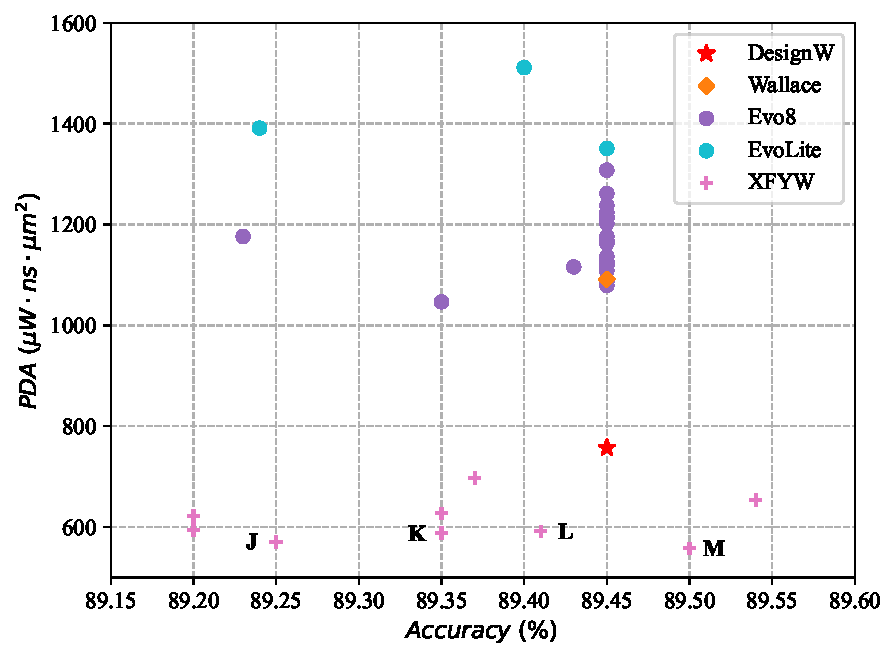
\includegraphics[width=0.9\linewidth]{figs/AC-AM-Adapt-VGG16_CIFAR-10_PDA_accuracy.pdf}
    \caption{不同乘法器在AlexNet和CIFAR-10上的精度以及2GHz时钟频率下的PDA散点图}
    \label{AC:AM:Adapt:Fig:VGG16_CIFAR-10_PDA_accuracy}
\end{figure}

图\ref{AC:AM:Adapt:Fig:VGG16_CIFAR-10_PDA_accuracy}展示了2个精确乘法器和多个近似乘法器在CIFAR-10\cite{DNN:CIFAR-10}和VGG16\cite{DNN:AlexNet}上的精度以及2GHz时钟频率约束下的PDA散点图,基于本文方法生成的XFYW乘法器的精度范围为$[89.2\%, 89.54\%]$,且有两个乘法器的精度高于精确乘法器,PDA优于图中出现的所有近似乘法器。
虽然基于CGP方法设计的Evo8\cite{AC:AM:CGP_Evoapprox8b}和EvoLite\cite{AC:AM:CGP_EvoLite}中部分乘法器精度尚可,但硬件成本显然比精确的DesignW乘法器高出数倍,这表明通过门级网表简化的办法在面向对误差容忍程度较低的应用时无法获得高性能的近似乘法器,违背了近似计算的初衷。
另外,基于$P=1$生成的XWYF乘法器没有出现在图\ref{AC:AM:Adapt:Fig:VGG16_CIFAR-10_PDA_accuracy}中,表明要么它们的准确率低于89.15\%要么具有非常差的PDA,这再一次证明了在设计非对称近似乘法器时考虑输入极性的重要性。与DesignW相比,乘法器\emph{`M'}的PDA改进了26.4\%,且精度更高(89.50\%)。选择\emph{`J'}、\emph{`K'}、\emph{`L'}、\emph{`M'}4个生成的近似乘法器与两个精确的乘法器进行进一步地比较,
\begin{figure}[!htb]
    \centering
    \includegraphics[width=0.7\linewidth]{figs/AC-AM-Adapt-VGG16_CIFAR-10_hist.pdf}
    \caption{基于VGG16和CIFAR-10的不同乘法器的功耗、延迟、面积、PDA和APDA,以DesignW为标准进行归一化}
    \label{AC:AM:Adapt:Fig:VGG16_CIFAR-10_hist}
\end{figure}
图\ref{AC:AM:Adapt:Fig:VGG16_CIFAR-10_hist}展示了6个乘法器在2GHz时钟频率约束下以DesignW为标准进行归一化后的功耗、延迟、面积、PDA和APDA对比图,可以看到与DesignW相比,4个近似乘法器的延迟稍差,意味着高频性能不足,但面积和功耗领先。乘法器$\emph{`M'}$的功耗、面积、PDA和APDA分别比DesignW好了22.1\%、6.4\%、26.4\%和33.1\%。

将图\ref{AC:AM:Adapt:Fig:VGG16_CIFAR-10_hist}中面向VGG16和CIFAR-10设计的XFYW近似乘法器分别放在LeNet和AlexNet中进行评估,其准确率分别为99.38\%-99.41\%和88.18\%-88.45\%,注意LeNet和AlexNet在精确乘法下的准确率分别是99.40\%和88.39\%,这再一次证明了针对大规模DNN设计的近似乘法器在面对小规模DNN时具有可迁移性。


\subsection{基于16比特补码有符号定点数的自适应FIR滤波器}

为了证明提出的方法对有符号乘法器同样有效,对基于16比特补码有符号定点数的自适应FIR滤波器进行数据分布特性分析并生成乘法器进行比较。
\begin{figure}[!ht]
    \centering
    \includegraphics[width=0.7\linewidth]{./figs/AC-AM-Adapt-FIR-structure.pdf}
    \caption{一个自适应FIR滤波器的结构图}
    \label{AC:AM:Adapt:FIR:Fig:structure}
\end{figure}
一个基本的自适应FIR滤波器的结构图如图\ref{AC:AM:Adapt:FIR:Fig:structure}所示,其中$n$代表迭代次数,$\boldsymbol{x}(n)$是输入向量,$\boldsymbol{w}(n)$是权重向量,由最小均方(Least Mean Squares, LMS)算法通过负反馈回路进行调整,$y(n)$是输出信号,$d(n)$是参考信号,$e(n)$是误差。
在$M$阶FIR滤波器中,假设第$n$次迭代时$\boldsymbol{w}(n) = [w_0(n), w_1(n), \cdots , w_{M-1}(n)]$,$\boldsymbol{x}(n) = [x(n), x(n-1), \cdots , x(n-M+1)]^\mathrm{T}$,输出信号$y(n)$由下式计算:
\begin{equation}
    \label{AC:AM:Adapt:FIR:Eq:yn}
    y(n) = \boldsymbol{w}(n) \cdot \boldsymbol{x}(n) = \sum_{0}^{M-1} w_i(n) \cdot x(n-i)
\end{equation}
误差$e(n)$为:
\begin{equation}
    \label{AC:AM:Adapt:FIR:Eq:en}
    e(n) = d(n) - y(n)
\end{equation}
权重向量由LMS算法进行调整,第$n+1$次迭代的第$i$阶权重$w_i (n+1)$为:
\begin{equation}
    \label{AC:AM:Adapt:FIR:Eq:LMS}
    w_i(n+1) = w_i(n) + \mu \cdot e(n) \cdot x(n-i)
\end{equation}
其中$i=0, 1, \cdots , M-1$,$\mu$代表步长。

自适应FIR滤波器由误差计算和权值更新两个模块组成,若阶数为$M$,则总共需要$2M$个乘法器。考虑一个基于16比特补码有符号数实现的20阶低通(Low pass)自适应FIR滤波器,LMS算法的步长为0.001,参考信号$d(n)$是一个叠加了高频噪声的幅值为5的正弦信号:
\begin{equation}
    \label{AC:AM:Adapt:FIR:Eq:dn}
    d(n) = 5 * sin ( \frac{\pi n}{25} ) + 0.5 * sin ( \frac{2 \pi n}{5}  + \frac{\pi}{4} )
\end{equation}
其中$n \in \{0, 1, \cdots, 999\}$,输入信号与噪声有一个$\dfrac{\pi}{4}$的相位差:
\begin{equation}
    \label{AC:AM:Adapt:FIR:Eq:xn}
    x(n) = sin ( \frac{2 \pi n}{5} )
\end{equation}

\begin{figure}[!ht]
    \centering
    \includegraphics[width=0.9\linewidth]{./figs/AC-AM-Adapt-FIR-weight_distribution.pdf}
    \caption{滤波器在精确乘法下的权重数据分布}
    \label{AC:AM:Adapt:FIR:Fig:weight_distribution}
\end{figure}

首先在精确乘法下运行滤波器并得到对应的权重数据,结果如图\ref{AC:AM:Adapt:FIR:Fig:weight_distribution}所示,可以看到分布是不均匀的。
假设$R=0.2$,由式\ref{AC:AM:Adapt:Eq:l_approx}得$l=6$,根据算法\ref{AC:AM:Adapt:Alg:lambda}得$P=0$和$P=1$下的$\lambda$下均为5000,基于式\eqref{AC:AM:Adapt:Eq:Obj}生成近似乘法器并进行PSNR的评估。

\begin{figure}[!ht]
    \centering
    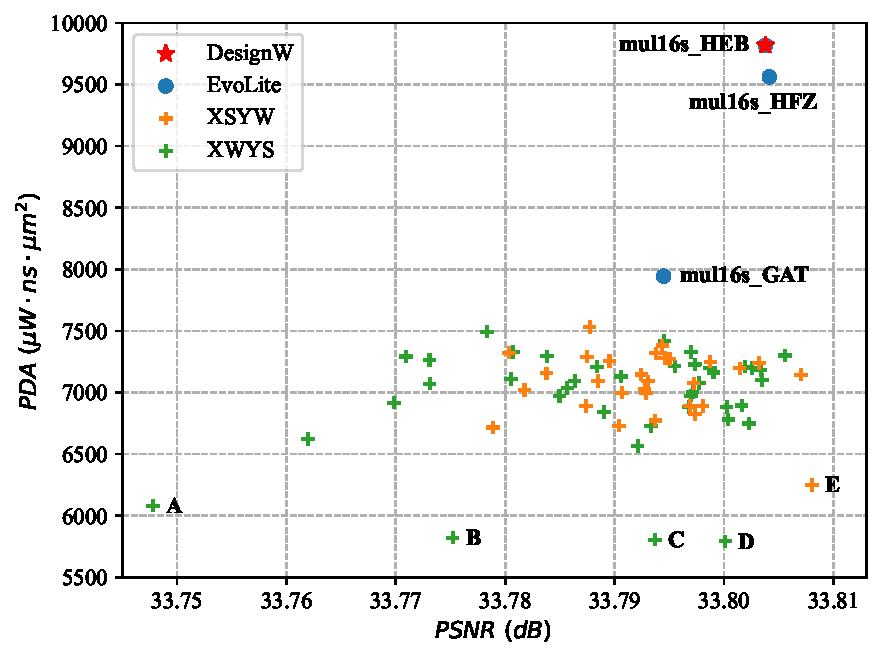
\includegraphics[width=0.9\linewidth]{./figs/AC-AM-Adapt-FIR-PSNR_PDA.pdf}
    \caption{不同乘法器的PDA和PSNR对比散点图}
    \label{AC:AM:Adapt:FIR:Fig:PSNR_PDA}
\end{figure}

图\ref{AC:AM:Adapt:FIR:Fig:PSNR_PDA}展示了不同乘法器基于1GHz时钟频率约束的PDA和PSNR对比散点图,其中DesignW代表DC通过DesignWare库\cite{IP:DesignWare}自动构建的16比特精确乘法器,XSYW和XWYS分别代表基于$P=0$($x$是信号输入,$y$是权重)和$P=1$($x$是权重,$y$是信号输入)生成的乘法器。
可以看到按照本文方法生成的近似乘法器在几乎没有PSNR损失的情况下提供了更好的PDA值,与DesignW和EvoLite中的mul16s\_GAT乘法器相比,5个生成的乘法器$\emph{`A'}$、$\emph{`B'}$、$\emph{`C'}$、$\emph{`D'}$、$\emph{`E'}$的PDA平均分别提升了41.0\%和27.1\%。

为了对不同乘法器的质量进行统一地比较,引入PDA和相对峰值信噪比损失的乘积(Product of PDA and relative PSNR loss, LPDA)来表征乘法器的好坏,相对PSNR损失被定义为:
\begin{equation}
    \lceil P_{exact} \rceil - P_{mul}
\label{AC:AM:Adapt:FIR:Eq:R_PSNR_Loss}
\end{equation}
其中$P_{exact}$代表滤波器在精确乘法器下的PSNR,$\lceil \ \rceil$代表向上取整,$P_{mul}$表示滤波器在某个乘法器下的PSNR,注意精确乘法器的相对PSNR损失不为0。

\begin{figure}[!ht]
    \centering
    \includegraphics[width=0.8\linewidth]{./figs/AC-AM-Adapt-FIR-hist.pdf}
    \caption{不同乘法器在200MHz时钟频率约束下的的功耗、延迟、面积、PDA和LPDA,以DesignW为标准进行归一化}
    \label{AC:AM:Adapt:FIR:Fig:hist}
\end{figure}

图\ref{AC:AM:Adapt:FIR:Fig:hist}展示了不同乘法器在200MHz时钟频率约束下以DesignW为标准进行归一化之后的的功耗、延迟、面积、PDA和LPDA对比图,可以看到mul16s\_GAT的功耗比DesignW低20\%左右,但面积没有很大优势。与mul16s\_GAT相比,根据本文的方法生成的5个乘法器的PDA和LPDA平均提升了12.5\%和8.3\%。


\subsection{半正态分布下的无符号32比特乘法器}

\begin{figure}[!htb]
    \centering
    \subfigure[$x$的直方图]{
    \label{AC:AM:Adapt:Fig:half-normal_32x32_x}
    \begin{minipage}[t]{0.48\linewidth}
    \centering
    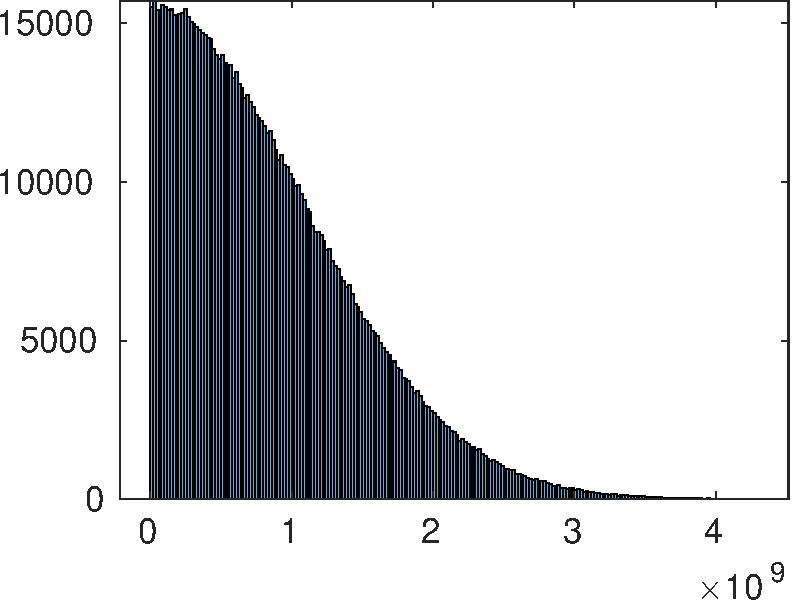
\includegraphics[width=\linewidth]{figs/AC-AM-Adapt-half-normal_32x32_x.pdf}
    \end{minipage}
    }
    \subfigure[$y$的直方图]{
    \label{AC:AM:Adapt:Fig:half-normal_32x32_y}
    \begin{minipage}[t]{0.48\linewidth}
    \centering
    \includegraphics[width=\linewidth]{figs/AC-AM-Adapt-half-normal_32x32_y.pdf}
    \end{minipage}
    }
\caption{基于平均值为0、标准差为$2^{30}$的正态分布随机生成的$2^{20}$对大于0的32比特输入数据直方图}
\label{AC:AM:Adapt:Fig:half-normal_histograms}
\end{figure}

\begin{figure}[!h]
    \centering
    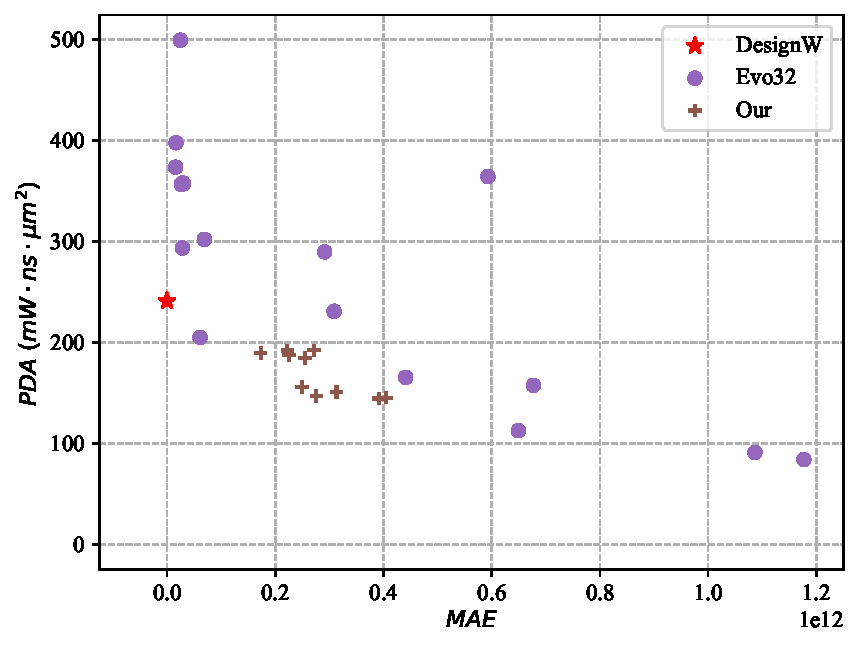
\includegraphics[width=0.8\linewidth]{figs/AC-AM-Adapt-half-normal_32x32_PDA_MAE.pdf}
    \caption{生成的近似乘法器与EvoLite中的32位无符号乘法器(Evo32)在1.5GHz时钟频率约束下进行MAE和PDA的比较}
    \label{AC:AM:Adapt:Fig:half-norm_32x32_PDA_MAE}
\end{figure}

为了验证方法在大位宽乘法器下的有效性,基于平均值$\mu$为0、标准差$\sigma$为$2^{30}$的正态分布(Normal distribution)随机生成了$2^{20}$对大于0的32比特输入数据(设为$x$和$y$),其直方图如图\ref{AC:AM:Adapt:Fig:half-normal_histograms}所示。
假设某一应用的乘法器也基于32比特的无符号数实现,且输入数据只从生成的$2^{20}$种情况中选择,精度由该$2^{20}$种情况下的平均绝对误差MAE(即平均误差距离MED,见式\eqref{AC:Arith:MED})决定。
考虑到$x$和$y$分布相同,所以无需考虑极性,且输入情况可以遍历。假设$R=0.15$,由式\eqref{AC:AM:Adapt:Eq:l_approx}得$l$取$10$,根据算法\ref{AC:AM:Adapt:Alg:lambda}确定$\lambda$为500后,求解\eqref{AC:AM:Adapt:Eq:Obj}得到近似乘法器。
在1.5GHz的时钟频率约束下与EvoLite\cite{AC:AM:CGP_EvoLite}中的32比特无符号乘法器(简称为Evo32)进行MAE和PDA的对比,结果如图\ref{AC:AM:Adapt:Fig:half-norm_32x32_PDA_MAE}所示,可以看到生成的乘法器与Evo32和DesignW一起组成了帕累拖前沿(Pareto front),证明了方法对大位宽乘法器的有效性。

\section{本章小结}


本章提出了一种由数据分布和输入极性驱动的自动化近似乘法器设计方法,该方法通过逻辑操作和移位操作对乘法器中的部分积在生成后、累加前进行压缩,以减轻后续的累加压力,达到降低电路硬件开销的目的。
基于均匀分布下的8比特无符号乘法器的实验结果表明,本文的方法生成的近似乘法器大幅优于已有的工作。
对LeNet、AlexNet和VGG16三种不同规模的基于8比特无符号数量化的DNN的实验结果表明,与最先进的近似乘法器相比,本文生成的乘法器在精度损失不超过0.01\%的情况下实现了26.4\%-47.6\%的PDA提升。同时,AlexNet和VGG16的实验结果证明了在设计非对称近似乘法器时考虑输入极性的重要性,也验证了基于提出的方法利用可迁移性为一类具有相似数据分布的应用生成一批近似乘法器的可行性。
对补码有符号乘法器的有效性在基于16位自适应LMS-FIR滤波器应用的实验中得到了证明,与国际前沿工作相比,生成的乘法器在PSNR损失可以忽略不计的情况下实现了PDA高达27.1\%的提升。
最后,基于32比特半正态分布的无符号数乘法器的实验结果表明,生成的乘法器与别的乘法器一起组成了帕累拖前沿,表明方法对大位宽乘法器同样有效。